%----------------------------------------------------------------------------------
% Exemplo do uso da classe pucrs-ppgcc.cls. Veja o arquivo .cls
% para mais detalhes e instruções.
%----------------------------------------------------------------------------------

% Seleção de idioma da monografia. Por enquanto as únicas opções
% suportadas são 'portuguese' e 'english'
% Para impressão em frente e verso, use a opção 'twoside'. Da
% mesma forma, use 'oneside' para impressão em um lado apenas.
\documentclass[portuguese,twoside]{pucrs-ppgcc}
%\documentclass[english,twoside]{pucrs-ppgcc}

%----------------------------------------------------------------
% Coloque seus pacotes abaixo.
%
% Obs.: muitos pacotes de uso comum do LaTeX, como amsmath,
% geometry e url já são automaticamente incluídos pela classe
% (veja o arquivo .cls). Isso torna obrigatória a presença destes
% no sistema para o uso desta classe, mas ao mesmo tempo o uso se
% torna mais simples.  Recomendo a instalação da versão mais
% recente da distribuição TeXLive (para Windows e UNIXes):
% www.tug.org/texlive/
%
% Pacotes e opções já incluídas automaticamente:
%
% \RequirePackage[T1]{fontenc}[2005/09/27]
% \RequirePackage[utf8x]{inputenc}[2008/03/30]
% \RequirePackage[english,brazil]{babel}[2008/07/06]
% \RequirePackage[a4paper]{geometry}[2010/09/12]
% \RequirePackage{textcomp}[2005/09/27]
% \RequirePackage{lmodern}[2009/10/30]
% \RequirePackage{indentfirst}[1995/11/23]
% \RequirePackage{setspace}[2000/12/01]
% \RequirePackage{textcase}[2004/10/07]
% \RequirePackage{float}[2001/11/08]
% \RequirePackage{amsmath}[2000/07/18]
% \RequirePackage{amssymb}[2009/06/22]
% \RequirePackage{amsfonts}[2009/06/22]
% \RequirePackage{url}
% \RequirePackage[table]{xcolor}[2007/01/21]
%----------------------------------------------------------------
% Para inserção de figuras.
\usepackage{graphicx}
% Utilize a opção 'pdftex' se você estiver usando o pdflatex (que
% permite figuras em formatos como .jpg ou .png)
%\usepackage[pdftex]{graphicx}

% Para tabelas com elementos ocupando mais de uma linha
\usepackage{multirow}
% Para frações na mesma linha (ex. ⅓).
\usepackage{nicefrac}
% Para inserir figuras lado a lado.
% \usepackage{subfigure}
% Para formatar algoritmos.
% A opção [algo2e] é necessária para evitar conflitos
% com as definições da classe.
%\usepackage[algo2e]{algorithm2e}
\usepackage{algorithmic}
% Um float do tipo algoritmo. No momento
% este pacote é incompatível com a classe.
% \usepackage{algorithm}
\usepackage{booktabs}

\author{Bruno Rubin dos Santos Matheus Bonifácio Morais}
\title{OLAP Docking - Uma solução OLAP para análise de experimentos de docagem molecular: aplicação com a enzima I\MakeLowercase{nh}A.}
      {OLAP Docking - An OLAP solution to analyze molecular docking experiments: applied to I\MakeLowercase{nh}A enzyme.}

\tipotrabalho{\monografia}  % Monografias em geral (e de "bônus": TCCs)
\grau{\bacharel} 

\orientador{Duncan Dubugras Alcoba Ruiz}

\begin{document}

%----------------------------------------------------------------
% Depois da capa vem a dedicatória e a epígrafe.
%----------------------------------------------------------------
%\dedicatoria{Dedico este trabalho a meus pais.}

%\epigrafe{The art of simplicity is a puzzle of complexity.}
%         {Douglas Horton}

%----------------------------------------------------------------
% Também dá para fazer as duas na mesma página:
%----------------------------------------------------------------
%\dedigrafe{Dedico este trabalho a meus pais.}
%          {The art of simplicity is a puzzle of complexity.}
%          {Douglas Horton}

%----------------------------------------------------------------
% A seguir, a página de agradecimentos (OPCIONAL):
%----------------------------------------------------------------
%\begin{agradecimentos}
%À lorem ipsum, dolor sit amet consetetur sadipscing elitr sed diam
%nonumy eirmod tempor. invidunt ut labore et dolore magna aliquyam
%
%À erad sed, diam voluptua at vero, eos et accusam et justo duo
%dolores et ea rebum stet clita.
%
%À kasd gubergren, no sea. takimata sanctus est lorem ipsum dolor sit
%amet lorem ipsum dolor sit amet. consetetur sadipscing elitr sed
%
%À diam nonumy, eirmod tempor, invidunt ut labore et dolore magna
%aliquyam erat sed diam voluptua at.
%\end{agradecimentos}

%----------------------------------------------------------------
% Resumo, com as palavras-chave passadas por parâmetro
% (OBRIGATÓRIO, ao menos para teses e dissertações)
%----------------------------------------------------------------
\begin{resumo}{OLAP, InhA, Docagem Molecular}

O processo de desenvolvimento de novos fármacos é uma atividade fundamental para a indústria farmacêutica, na qual é utilizado não somente para o desenvolvimento de novos compostos para atender uma determinada necessidade, mas também tem como objetivo evoluir os compostos já existentes em busca de um resultado aprimorado e mais eficaz. A área de bioinformática tem como um de seus objetivos, através do uso de recursos e técnicas computacionais, acelerar e aprimorar o processo de desenvolvimento de medicamentos.
Esse processo consiste na análise das interações entre pequenas moléculas e receptores, e o processo de docagem molecular, é o responsável por simular e avaliar de forma qualitativa as interações estabelecidas.  O principal desafio para a realização destes experimentos é quando a flexibilidade do receptor é considerada. Para este caso, é utilizado um conjunto de conformações (snapshots) gerados apartir de simulações por dinâmica molecular.
A análise dos dados resultantes de docagem é feita de forma manual pelo especialista de domíno através do uso de um protocolo para avaliação. Os dados gerados pelas simulações crescem de acordo com o conjunto de snapshots que é utilizado, dificultando a análise e visualização de todos os resultados. 

\end{resumo}

%----------------------------------------------------------------
% Abstract, com as palavras-chave passadas por parâmetro
% (OBRIGATÓRIO, ao menos para teses e dissertações)
%----------------------------------------------------------------
\begin{abstract}{lorem, ipsum, dolor, sit, amet}
Your abstract in English here. lorem ipsum dolor sit amet
consetetur sadipscing elitr sed diam nonumy eirmod tempor invidunt
ut labore et dolore magna aliquyam erat sed diam voluptua at vero
eos et accusam et justo duo dolores et ea rebum stet clita kasd
gubergren no sea takimata sanctus est lorem ipsum dolor sit amet
lorem ipsum dolor sit amet consetetur sadipscing elitr sed diam
nonumy eirmod tempor invidunt ut labore et dolore magna aliquyam
erat sed diam voluptua at
\end{abstract}

%----------------------------------------------------------------
% Listas e sumário, nessa ordem. Somente o sumário é obrigatório,
% portanto, comente as outras listas, caso sejam desnecessárias.
%----------------------------------------------------------------
\listoffigures       % Lista de figuras      (OPCIONAL)
\listoftables        % Lista de tabelas      (OPCIONAL)
%\listofalgorithms    % Lista de algoritmos   (OPCIONAL)
\listofacronyms      % Lista de siglas       (OPCIONAL)
%\listofabbreviations % Lista de abreviaturas (OPCIONAL)
%\listofsymbols       % Lista de símbolos     (OPCIONAL)
\tableofcontents     % Sumário               (OBRIGATÓRIO)


\sigla{3D}		{Tridimensional}
\sigla{BD}		{Banco de Dados}
\sigla{CADD}	{\emph{Computer-aided drug design} ou desenvolvimento de fármacos auxiliado por computador}
\sigla{DM}		{Dinâmica Molecular}
\sigla{ETH}		{Etionamida}
\sigla{FEB}		{\emph{Free Energy of Binding} ou Energia Livre de Ligração}
\sigla{InhA}	{Enzima 2-trans-Enoil ACP(CoA) Reductase de Mycobacterium tuberculosis }
\sigla{LABIO}	{Laboratório de Bioinformática, Modelagem e Simulação de Biossistemas}
\sigla{NADH}	{Resíduo Nicotinamida Adenina Dinucleotídeo}
\sigla{PDB}		{\emph{Protein Data Bank} ou Banco de Dados de Proteínas}
\sigla{RDD}		{\emph{Rational Drug Design} ou Planejamento Racional de Fármacos}
\sigla{RMSD}	{\emph{Root Mean Square Deviation} ou Desvio Médio Quadrático}
\sigla{TCL} 	{Triclosano}
\sigla{CSV} 	{\emph{Comma-separated values}}
\sigla{OLAP} 	{\emph{Online Analytical Processing}}
\sigla{SQL} 	{\emph{Structured Query Language}}
\sigla{CLI} 	{\emph{Command-line interface}}
\sigla{STDOUT} 	{\emph{Standard output}}



%----------------------------------------------------------------
% Aqui começa o desenvolvimento do trabalho. Para uma melhor
% organização do documento, separe-o em arquivos,
% um para cada capítulo. Para isso, utilize o comando \include,
% como mostrado abaixo.
%----------------------------------------------------------------
\chapter{Introdução}
\section{Caracterização do problema}
O processo de desenvolvimento de novos fármacos é uma atividade fundamental para a indústria farmacêutica, na qual é utilizado não somente para o desenvolvimento de novos compostos para atender uma determinada necessidade, mas também tem como objetivo evoluir os compostos já existentes em busca de um resultado aprimorado e mais eficaz. 

Este processo possui uma alta complexidade e exige, em média, 14 anos desde a identificação até a liberação pelo órgão regulador. As etapas envolvidas neste processo vão desde a identificação de um possivel candidato à fármaco, seguido por uma pesquisa de otimização, testes \emph{in-silico} e \emph{in-vitro}, análises toxicológicas até os ensaios clínicos. Estima-se que os custos de desenvolvimento de um novo fármaco seja aproximadamente de 1,2 bilhões de dólares \cite{kun92}. 

A área de bioinformática tem como um de seus objetivos, através do uso de recursos e técnicas computacionais, auxiliar o processo de descobrimento de novos fármacos. A partir de algoritmos computacionais é possível realizar simulações para identificar possíveis candidatos a novos fármacos e, posteriormente, submetê-los a testes mais específicos. Estes testes e simulações executados com auxílio computacional são denominados \emph{in-silico}.

O fator de desenvolvimento constante de novos \emph{softwares} e \emph{hardwares} contribui para que experimentos deste tipo sejam executados de forma cada vez mais rápida e com um maior nível de precisão. Esta metodologia passou a ser utilizada exaustivamente pelas indústrias farmacêuticas por se tratar de um método que exige um menor custo financeiro, se comparado com os tradicionais testes em laboratório \cite{art08}. 

O LABIO (Laboratório de Bioinformática, Modelagem e Simulação de Biossistemas) da Faculdade de Informática da Pontifícia Universidade 
Católica do Rio Grande do Sul (PUCRS) realiza pesquisas e estudos \emph{in-silico} de interações entre a enzima InhA (\emph{Mycobacterium 
tuberculosis}) e seus resíduos, que possam apresentar ligações receptor-ligante estáveis através de simulações de docagem molecular.

Dentro do processo de desenvolvimento de fármacos, a docagem molecular pode ser considerada como o principal método para avaliar a eficácia das combinações químicas entre as conformações. A docagem molecular é um método a qual prediz a orientação preferencial de encaixe de uma molécula à outra, com o objetivo de formar um complexo receptor-ligante estável. Este método pode ser simulado computacionalmente através dos algoritmos de docagem. 

A docagem basicamente envolve duas moléculas, uma chamada de receptor, que normalmente é uma proteína, e um ligante que á a molécula complementar que se conecta ao receptor. A avaliação do resultado da ligação estabelecida entre as duas moleculas se dá pelo cálculo de duas propriedades, uma é chamada de energia livre de ligação (Free energy of binding) e a outra é chamada de RMSD (Root mean square deviation). Analisar esta interação entre o receptor e o ligante não é uma tarefa simples visto que estes são influenciados por uma série de fatores ambientais. Os algoritmos de docagem precisam levar em consideração todas as formas de ligação entre o ligante e o receptor, o que inclui a exploração de todos os graus de liberdade translacionais e rotacionais do ligante, além dos graus de liberdade conformacionais do receptor.

O principal desafio da realização de testes \emph{in-silico} é quando a flexibilidade da molécula receptora passa a ser considerada. Devido ao tamanho da molécula e sua complexidade, as simulações com receptores flexíveis requerem um grande esforço computacional para realização dos cálculos necessários \cite{art08}.
Existem diversas abordagens para contornar este problema, e uma delas é a utilização de conjuntos de conformações gerados em simulações por Dinâmica Molecular (DM). Esta técnica consiste em gerar um conjunto de conformações de uma proteina em um intervalo de tempo, tendo como objetivo principal o estudo do comportamento dinâmico e também da geometria de uma proteína. Cada conformação em um instante de tempo específico é denominada \emph{snapshot} e possui propriedades que podem ser calculadas. Com isso, é executado uma simulação de docagem molecular para cada \emph{snapshot} do conjunto gerado por DM.

Todavia, apesar das metologias que geram um conjunto de conformações representativas do comportamento dinâmico de um receptor, a análise dos dados resultantes das simulações de docagem molecular ainda se faz de forma manual pelo especialista de domíno. A análise das interações ligante-receptor acaba se tornando humanamente inviável de ser feita para todos os resultados da docagem, pois o especialista possui um protocolo utilizado para avaliar de forma manual estes resultados, através dos valores de FEB (Free Energy of Binding) e RMSD (Root-mean-square Deviation), e também a geometria resultante.

Estima-se que a análise dos dados resultantes, seguindo o protocolo utilizado pelo especialista, necessitaria de aproximadamente 516 horas (mais de 21 dias) para ser concluída para todos os resultados de apenas uma molécula ligante, se fosse utilizado uma dinâmica molecular de 3.100 conformações (levando em consideração o tempo médio de análise de 10 minutos por conformação). Este número se torna ainda mais expressivo para uma simulação utilizando uma dinâmica molecular de 20.000 conformações, atualmente em uso no LABIO.


\section{Motivação}

Dados da Organização Mundial da Saúde confirmam que a Tuberculose (TB) é a segunda doença infecciosa que mais causa mortes em todo o mundo, perdendo apenas para o HIV/AIDS. No ano de 2012, 8.6 milhões de pessoas foram diagnosticadas com Tuberculose e 1.3 milhões morreram por estarem infectadas. A Tuberculose, causada pela bactéria \emph{Mycobacterium tuberculosis}, embora seja curável, é uma preocupação de nível mundial.

Atualmente existem programas governamentais que se esforçam no controle e no combate à TB, que tem como objetivo principal evitar que a doença seja difundida entre a população. Para o tratamento da doença, existem três principais fármacos que são utilizados: isoniazida (INH), rifampicina (RMP) e pirazinamida (PZA). O tratamento realizado com estes fármacos tem duração, em média, de 6 meses. Se não houver colaboração do paciente e o tratamento for interrompido de forma precoce, pode gerar bactérias resistentes à estes compostos químicos, sendo mais difíceis de combater. Devido aos efeitos colaterais destes medicamentos, muitas vezes o tratamento não é concluído adaquadamente, criando bactérias mais resistentes.

O desenvolvimento de novos fármacos ou a melhoria de compostos químicos já existentes é um esforço necessário para controle e combate a Tuberculose. O processo de CADD, desenvolvimento de fármacos auxiliado por computador (do inglês \emph{Computer-aided drug design}), é utilizado em larga escala para testes \emph{in-silico}, com objetivo de identificar novos compostos que mostrem eficácia e minimizem os efeitos colaterais aos pacientes.

Além da motivação relacionada ao receptor InhA que está sendo utilizado neste trabalho, uma das principais motivações está em contribuir com a comunidade de bioinformática e com o LABIO da PUCRS na pesquisa e desenvolvimento de métodos para cura e controle desta doença, através do desenvolvimento de uma ferramenta que auxilie a análise dos dados resultantes de experimentos realizados. 

Poranto, a utilização da ferramenta desenvolvida neste trabalho permitirá ao especialista de domínio uma maior chance de identificar ligações estáveis em um menor período de tempo, sem que haja conhecimentos avançados de informática e sem necessitar de recursos computacionais de alta capacidade.

\section{Objetivos}
\subsection{Objetivo geral}
O objetivo deste trabalho é contribuir com a análise dos resultados de simulações de docagem molecular através do desenvolvimento de um modelo OLAP e de todo o processo de extração, transformação e carga de dados, de forma a organizar estes resultados sob uma estrutura de cubos, e possibilitar, ao especialista de domínio, a realização de uma análise multidimensional das informações ali presentes e a obtenção de informações relevante de uma maneira mais rápida e menos custosa.

\subsection{Objetivos específicos}
\begin{itemize}
	\item Desenvolver um conjunto de scripts para preparação de dados de simulações de docagem molecular para carga no modelo OLAP.
	\item Desenvolver um modelo OLAP baseado em um banco de dados utilizado para armazenamento de resultados de docagem molecular.
	\item Permitir aos especialistas de domínio o cruzamento das informações de uma simulação por agrupamento de conformações.
	\item Contribuir para que os resultados das simulações de docagem molecular possam ser analisados multidimensionalmente, facilitando a identificação de complexos receptor-ligantes estáveis.
\end{itemize}

\section{Organização do documento}

Este documento está organizado da seguinte maneira:

\begin{itemize} 
	\item O Capítulo 2 apresenta os conceitos fundamentais para entendimento do trabalho desenvolvido, como: planejamento racional de fármacos, dinâmica molecular e o processo de docagem molecular. Ainda neste capítulo são apresentados conceitos de modelos multidimensionais OLAP e processo de ETL.
	\item No Capítulo 3 são apresentadas breves descrições das ferramentas que foram empregadas para o desenvolvimento deste trabalho, como a linguagem Python e o Microsoft SQL Analysis Services respectivamente.
	\item O Capítulo 4 descreve os elementos envolvidos na modelagem deste trabalho, bem como a fonte de dados utilizada para extração das informações.
	\item No Capítulo 5 são apresentadas todas as etapas envolvidas no processo de desenvolvimento do trabalho, desde identificação de métricas utilizadas, desenvolvimento de scripts para processo de ETL, concepção e definição das dimensões do modelo multidimensional, até por fim apresentar a construção do modelo OLAP em si.
	\item O Capítulo 6 apresenta as questões de negócio que foram possíveis responder utilizando o modelo OLAP desenvolvido e também as possibilidades de consultas e análise multidimensional dos dados.
	\item No Capítulo 7 são apresentadas as conclusões deste trabalho e também sugere algumas possibilidades para trabalhos futuros.
	
\end{itemize} 
% ----------------------------------------------------------
% Referencial Teórico
% ----------------------------------------------------------
\chapter{Referencial Teórico}

\section{Planejamento Racional de Fármacos}
Devido aos avanços da biologia, atualmente o processo de descoberta e desenvolvimento de novos compostos químicos capazes de prevenir ou curar doenças passou a seguir um planejamento racional, com embasamento lógico e teórico \cite{rdd}. Esse processo é denominado “Planejamento Racional de Fármacos” (do inglês RDD - \emph{Rational Drug Design}) e, de acordo com Kuntz \cite{kun92}, ele se divide em quatro etapas e está reprensentados através do \emph{workflow} da Figura \ref{fig:rddworkflow} \cite{kar11}: 

\begin{figure}[h]
	\center
	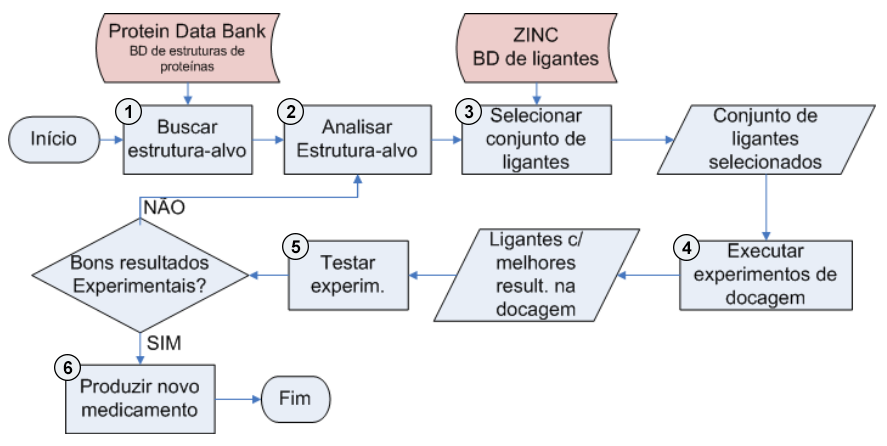
\includegraphics[width=14cm]{images/rdd_workflow.png}
	\label{fig:rddworkflow}
	\caption{\emph{Workflow} do processo de planejamento racional de fármacos assistido por computador \cite{kar11}}
\end{figure}


\begin{enumerate}
  \item O primeiro passo é definir um receptor (normalmente uma proteína) \cite{dre00} e analisar computacionalmente sua estrutura 3D. A estrutura da proteína é determinada por cristalografia por difração de raios X ou ressonância magnética nuclear \cite{far99}, sendo as informações resultantes armazenadas em um banco de dados como o Protein Data Bank - PDB \cite{ber00}. Essa análise tem por objetivo localizar possíveis regiões de ligação onde um ligante pode estabelecer ligações (atividades 1 e 2 do \emph{workflow} da Figura \ref{fig:rddworkflow});
  
  \item Baseado nas prováveis regiões de ligação identificadas no passo anterior, é selecionado um conjunto de possíveis candidatos, chamados ligantes (usualmente pequenas moléculas que podem ser buscadas em Banco de Dados de compostos como o ZINC \cite{irw05}) que podem se ligar a essa região no receptor (atividade 3 \emph{workflow} da Figura \ref{fig:rddworkflow}). As diferentes conformações que determinado ligante pode assumir dentro do sítio de ligação de uma determinada proteína são simuladas por softwares de docking como AutoDock 3.05 \cite{mor98} (atividade 4 do \emph{workflow} da Figura \ref{fig:rddworkflow});
  
  \item Os ligantes que teoricamente obtiveram melhores resultados nas simulções são experimentalmente sintetizados e testados (atividade 5 do \emph{workflow} da Figura \ref{fig:rddworkflow});
  
  \item Baseado nos resultados experimentais, o medicamento é gerado (atividade 6 do \emph{workflow} da Figura \ref{fig:rddworkflow}) ou o processo retorna ao passo 1.
  
\end{enumerate}
  
  Estas quatro etapas descritas por Kuntz \cite{kun92} contemplam apenas as fases de pesquisa e desenvolvimento de um novo medicamento. 
Somente após um longo período de pesquisas e testes \emph{in-vitro} e \emph{in-vivo}, estabelecendo eficácia e segurança, o novo fármaco é submetido para registro no órgão regulador.

A Tabela \ref{tab:rddtempo} apresenta, de uma forma geral, as etapas que envolvem o processo de desenvolvimento de um novo fármaco e o tempo médio de cada uma delas \cite{kun92}.

% Please add the following required packages to your document preamble:
% \usepackage{booktabs}
\begin{table}[h]
	\caption{Passos e tempo para desenvolvimento de um novo fármaco \cite{kun92}}
	\label{tab:rddtempo}
	\centering
	\begin{tabular}{@{}lc@{}}
	\toprule
	\multicolumn{1}{c}{\textbf{Passo}}      & \textbf{Tempo (Anos)} \\ \midrule
	Descoberta e geração de um candidato    & 1 - 2                 \\
	Otimização do candidato                 & 1 - 2                 \\
	Ensaios in-vitro e in-vivo              & 1 - 2                 \\
	Testes toxicológicos                    & 1 - 3                 \\
	Testes de segurança em humanos          & 1                     \\
	Testes de eficiência em humanos         & 1 - 2                 \\ \midrule
	\textbf{Tempo total de desenvolvimento} & \textbf{6 - 12}       \\ \bottomrule
	\end{tabular}
\end{table}

O desenvolvimento de fármacos auxiliado por computador (do inglês CADD - \emph{Computer-aided drug design}) consiste na utilização de recursos, ferramentas e técnicas computacionais contribui de forma significativa para as etapas de desenvolvimento de um fármaco.  Diferentes estágios deste processo podem ser beneficiados pelo uso da computação, podendo ser aplicado na identificação da molécula-alvo, planejamento, análise e melhoramento de ligantes.


\section{Dinâmica Molecular}

O advento da utilização de recursos computacionais aplicado às áreas medicinais e biológicas têm proporcionado o avanço de técnicas e uso de ferramentas que contribuem de forma expressiva para o planejamento racional de fármacos.

A Dinâmica Molecular (DM) é uma técnica de simulação computacional, fundamentada nos princípios da Mecânica Clássica, que possibilita o estudo do comportamento dinâmico microscópico de um sistema molecular, em diferentes intervalos de tempo \cite{nam08}. 

A simulação por DM fornece informações dos átomos que constituem o sistema molecular, permitindo o cálculo de diversas propriedades (pressão, temperatura, volume, energia livre, etc) e análise do potencial de interação dos ligantes na estrutura e estabilidade das proteínas \cite{kar11}.

De acordo com Lesk \cite{art08}, as interações entre os átomos em uma molécula podem ser classificadas de duas maneiras:

\begin{quote}
	(a) Ligações químicas primárias - interações fortes entre átomos que estão localizados bem próximos no espaço. São consideradas interações fixas pois são consistentes em um grande número de conformações, não sendo desfeitas ou alteradas quando a conformação de uma proteína muda. 

	(b) Interações mais fracas que dependem da conformação, podem ser significativas em algumas conformações e não em outras - elas afetam conjuntos de átomos que são aproximados devido a diferentes padrões de enovelamento da cadeia.
\end{quote}

As proteínas são corpos flexíveis que não possuem uma conformação única e fixa. Elas apresentam conformações que variam em um intervalo de tempo. A Figura \ref{fig:dm} ilustra a flexibilidade da enzima receptora InhA, onde cada cor representa uma conformação em um determinado instante de tempo \cite{COH10}.

\begin{figure}[h]
	\center
	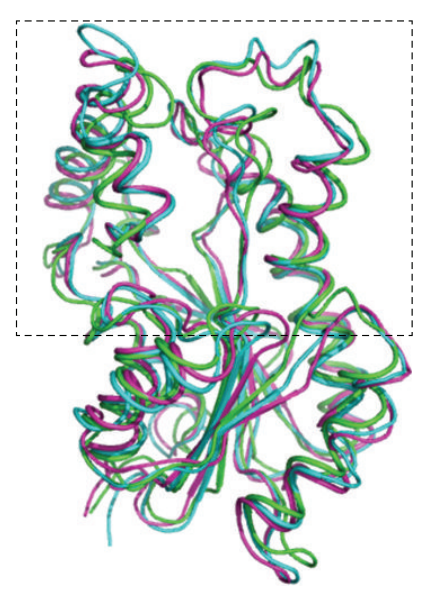
\includegraphics[width=14cm]{images/dm_inha.png}
	\label{fig:dm}
	\caption{Flexibilidade da enzima receptora InhA. Sobreposição de diferentes conformações da InhA, representadas em fitas, durante uma simulação de DM. A conformação inicial da simulação está representada pela cor verde. Outras duas conformações foram capturadas pela simulação de DM nos intervalos de 1,000 ps (cor azul) e 3,000 ps (cor magenta). O retângulo tracejado identifica a região com maior flexibilidade \cite{REN13}.}
\end{figure}

A conformação de uma proteína pode ser especificada pela lista de átomos na estrutura, por suas coordenadas e pelo conjunto de ligações químicas entre eles. A avaliação de uma conformação é feita através do cálculo de conjuntos de potenciais de energia. Estes calculos são computacionalmente complexos e intensivos, mas com a evolução rápida da capacidade de processamento dos computadores esta técnica é beneficiada diretamente \cite{art08}.

A simulação por DM se mostra um método versátil e acessível, sendo considerada a melhor técnica para geração de um conjunto de conformações de um receptor \cite{kar11}. Devido à isso, os dados dos conjuntos de conformações dos receptores utilizados neste trabalho foram gerados utilizando a DM.


\section{Docagem Molecular}

A Docagem Molecular é considerada um dos principais processo do CADD, e é através dela que são produzidos os dados detalhados sobre a interação entre receptores e seus ligantes \cite{LEN96}. 

No processo de Docagem Molecular, algoritmos de docagem são executados para testar e analisar virtualmente a interação entre um ligante e um receptor. Estes algoritmos geram um grande número de interações, onde em todas elas, o ligante é testado em diferentes orientações e conformações dentro do sítio de ligação do receptor, de modo a formar um complexo estável. 
Usualmente o receptor é uma proteína ou uma molécula de ácido nucléico, e o ligante pode ser uma pequena molécula ou até mesmo outra proteína. A Figura \ref{fig:docking} \cite{ALE13} ilustra cada um destes elementos e apresenta como é feita a interação entre eles.

\begin{figure}[h]
	\center
	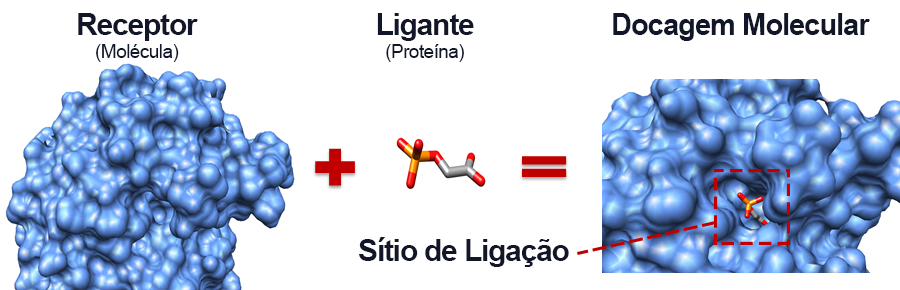
\includegraphics[width=14cm]{images/docking.png}
	\label{fig:docking}
	\caption{Representação do processo de docagem molecular em três dimensões (3D) entre uma proteína como receptor e uma pequena molécula como ligante, na qual se estabelece uma interação entre eles no sítio de ligação do receptor \cite{ALE13}.}
\end{figure}

Diversas interações devem ser testadas para que seja identificado o melhor encaixe do ligante no sítio de ligação do receptor, ou então, a região ou o sítio de ligação deve ser previamente conhecido. Um dos critérios utilizados para avaliar as interações é pelo cálculo da energia livre de ligação (do inglês FEB - \emph{Free Energy of Binding}). Quanto mais negativo for o valor resultante, melhor é a ligação estabelecida \cite{kar07}. A Figura \ref{fig:TCLdocking} \cite{REN13} ilustra o processo de docagem em três dimensões, a posição inicial da molécula do ligante TCL no sítio de ligação da molécula InhA e a posição do ligante TCL após a simulação de docagem molecular.

\begin{figure}[h]
	\center
	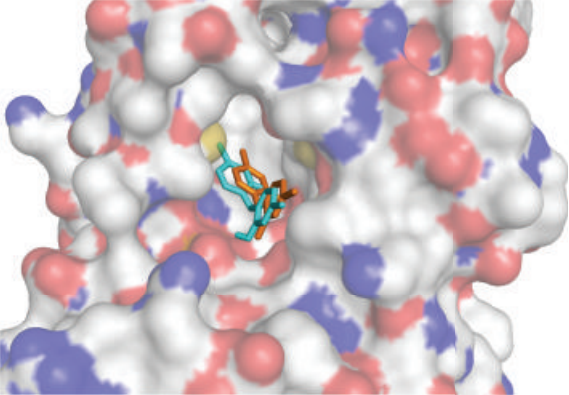
\includegraphics[width=14cm]{images/TCLdocking.png}
	\label{fig:TCLdocking}
	\caption{Representação da superfície molecular do sítio de ligação da enzima receptora InhA na estrutura de cristal. O ligante TCL é  representado na forma de palitos. A conformação inicial do ligante TCL aparece em cor laranja, e a conformação final após uma simulação de docagem molecular é representada em ciano \cite{REN13}.}
\end{figure}

As primeiras abordagens envolvendo a docagem entre proteínas e ligantes consideravam ambos elementos como sendo corpos rígidos. O modelo conhecido como "chave e fechadura" (do inglês \emph{lock-and-key}, proposto por Emil Fisher em 1894, prevê um encaixe perfeito do ligante no sítio de ligação do receptor, tal como uma chave encaixa em sua fechadura correspondente \cite{kar07}. 

No entanto, ambos proteína e ligante são moléculas flexíveis. Desta forma, o modelo histórico de "chave e fechadura" deu seu lugar à novas teorias, as quais passaram a considerar totalmente ou parcialmente a flexibilidade do ligante e do receptor \cite{SOU06}. Atualmente um dos maiores desafios na área de docagem molecular é conseguir manipular, de forma eficience, a flexibilidade do receptor da proteína. A eficiência da busca pela melhor conformação é determinada pelo número de graus de liberdade  \cite{SOU06}. 

Considerar a flexibilidade do ligante não requer um grande esforço computacional, pois geralmente são moléculas pequenas que possuem poucos átomos em sua estrutura \cite{COH10}. No entanto, a consideração da flexibilidade de ambos receptor e ligante se torna um complicador para os cálculos da docagem molecular, se tornando um problema computacional devido a complexidade e ao tamanho da proteína receptora \cite{art08}.

Existem diversos estudos e abordagens que contemplam a flexibilidade do receptor em simulações de docagem molecular. Entretanto, no presente trabalho, os dados utilizados foram previamente desenvolvidos no LABIO (Laboratório de Bioinformática, Modelagem e Simulação de Biossistemas) combinando técnicas de docagem molecular com dados resultantes de simulações por DM. A partir disso, foi gerado um conjunto de \emph{snapshots} sequenciais que representam as diferentes conformações da proteína receptora InhA em um intervalo de tempo.bilidade do ligante \cite{kar11}.

\section{Modelagem OLAP}

Com o desenvolvimento tecnológico, ficou cada vez mais fácil a obtenção de dados sobre um determinado assunto. Atualmente, qualquer aparelho eletrônico é capaz de gerar uma imensa massa de dados. Porém, estes dados se tornam irrelevantes se não estiverem devidamente organizados e não possuirem uma ferramenta capaz de tratá-los. Para as organizações, o tratamento destes dados significa transformá-los em algo que possa agregar valor.

Um sistema de suporte à decisão (do inglês OLAP - \emph{On-line Analytical Processing}) é uma ferramenta que permite analisar os dados \emph{on-line} de forma multidimensional, auxiliando a tomada de decisão nos mais diversos níveis, sejam eles operacionais, táticos e estratégicos. De acordo com com Turban \emph{et al.} \cite{TUR05}, o OLAP se define em “uma categoria ampla de aplicações e técnicas para coletar, armazenar, analisar, fornecer acesso aos dados e ajudar os usuários da empresa a fazerem melhores negócios e tomarem melhores decisões estratégicas”. 

A representação dos dados em um modelo OLAP é como uma matriz. Cada dimensão é caracterizada por uma questão de negócio e sempre considera-se uma dimensão para o tempo. Também é possível que uma dimensão possua hierarquia, por exemplo, a dimensão tempo pode ter: ano, semestre, mês, dia, etc. Nestas dimensões os dados são agregados, mas é possível navegar entre as hierarquias de modo que os dados sejam exibidos com um maior nível de granularidade. A ação de ir de um nível genérico para um mais detalhado é chamado de \emph{drill-down}. A ação inversa é chamada de \emph{drill-up}.

Um modelo dimensional implementado em um banco de dados relacional é representado fisicamente por tabelas, e caracteriza-se pelo modelo do tipo estrela (do inglês \emph{Star Schema}) devido à forma que a sua estrutura está organizada. Este tipo de modelo possui como principal característica o relacionamento entre diversas tabelas de dimensão e uma tabela de fatos centralizada \cite{KIM13}.

Quando o modelo dimensional passa a ser implementado em um banco de dados multidimensional, sua representação é na forma de um cubo. Um cubo OLAP pode ser equivalente ou derivado de um modelo do tipo estrela \cite{KIM13}. A Figura \ref{fig:starVSolap} ilustra a organização estrutural dos dados utilizando o modelo estrela e o modelo em cubo.

\begin{figure}[h]
	\center
	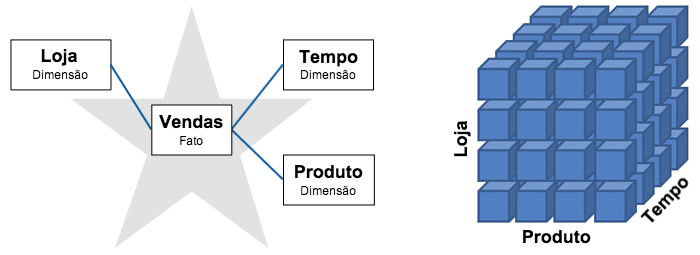
\includegraphics[width=14cm]{images/starvsolap.png}
	\label{fig:starVSolap}
	\caption{Representação da organização estrutural dos dados nos modelos do tipo estrela e cubo. (Material adaptado de \cite{KIM13})}
\end{figure}

As dimensões representam os elementos "quem, o quê, onde, quando, como e porquê" de um processo de negócio de uma organização, por exemplo: "produto", "vendedor" e "loja". Cada dimensão possui uma chave primária e um conjunto de atributos que descrevem de forma textual os elementos envolvidos no processo de negócio. Os atributos servem para detalhar as características de uma dimensão e são essenciais para auxiliar na tomada de decisão \cite{KIM13}. Utilizando como exemplo a dimensão "produto", ela poderia conter os atributos "nome", "preço" e "categoria".

A tabela fato é onde as informações produzidas pela execução de um processo de negócio são armazenadas. Estas informações são chamadas de métricas ou medidas. As métricas geralmente são valores numéricos, pois os dados são agregados utilizando operações de somatório, média, etc. Cada entrada em uma tabela fato, corresponde a uma entrada em cada uma das dimensões \cite{KIM13}. A Figura \ref{fig:exOlap} ilusta um modelo relacional do tipo estrela.

\begin{figure}[h]
	\center
	\includegraphics[width=14cm]{images/exOlap.png}
	\label{fig:exOlap}
	\caption{Representação de um modelo dimensional em um banco de dados relacional do tipo estrela.}
\end{figure}

Os dados armazenados em um cubo OLAP passam por algoritmos de indexação, técnicas de armazenamento e outras otimizações que fazem com que as consultas realizadas nesta estrutura de dados, mesmo sendo complexas, tenham um alto desempenho no tempo de resposta para o usuário.

Um dos processo que fazem parte da modelagem de dados OLAP é o de extração, transformação e carga (do inglês ETL - \emph{Extract, Transform and Load}). Este processo consiste na extração de dados de fontes externas e na transformação dos mesmos, para que possam atender às necessidades de negócio. Posteriormente, estes dados são carregados em um \emph{Data Warehouse} ou em outros ambientes de banco de dados.

O processo de ETL é considerado o mais complexo e que consome mais tempo durante a criação de um ambiente de \emph{Data Warehouse/Business Intelligence}, pois consiste em movimentar e transformar os dados que irão servir como base para futuras decisões gerenciais. Portanto, os dados precisam estar precisos e consistentes. Muitas vezes as informações estão armazenadas em diferentes fontes de dados e não possuem um padrão de estrutural de dados \cite{kim13}. Nestes casos, as etapas de extração e transformação precisam de um esforço para que os dados sejam tratados de forma homogênea.
























% ----------------------------------------------------------
% Ferramentas de Desenvolvimento
% ----------------------------------------------------------
\chapter{Ferramentas de Desenvolvimento}

\section{Linguagem Python}
A escolha da linguagem Python foi uma peça-chave para possibilitar o desenvolvimento de um script para preparação dos dados. Uma simulação de docagem molecular gera um alto volume de dados, e para tratá-los, foi necessário a utilização de uma linguagem que suportasse esta carga e apresentasse uma forma simples de desenvolvimento.

A linguagem Python é uma linguagem na qual possui uma curva de aprendizado relativamente simples se comparada com as outras linguagens utilizadas no mercado, isto se deve ao fato de o Python possuir uma estrutura de dados mais alto nível e uma abordagem simples, mas efetiva para programação orientada à objeto. Por possuir uma sintaxe clara e de tipagem dinâmica, se torna simples a compreensão \cite{pyt00}. 

Outra característica da linguagem Python é ser multiplataforma. É possível a execução em ambientes Windows, Mac e todas as distribuições Linux. Esta característica contribui para que programas escritos nesta linguagem sejam portáveis para qualquer outra plataforma com facilidade \cite{pyt01}.

A biblioteca padrão da linguagem Python possui módulos nativos para processamento de texto e expressões regulares. Observando à estas características, o Python apresentou-se como uma linguagem ideal para ser empregada neste tipo de problema. 

\section{SQL Server Analisys Services}
	explicar didaticamente sobre o que é e pra que serve
\chapter{Materiais utilizados}

\section{Receptor Investigado}

A Tuberculose, causada pela bactéria \emph{Mycobacterium tuberculosis}, é a segunda doença infecciosa que mais causa mortes em todo o mundo. 

O tratamento com os principais fármacos utilizados atualmente tem duração, em média, de 6 meses e apresenta diversos efeitos colaterais. Muitas vezes o paciente interrompe precocemente o tratamento, propiciando o surgimento de bactérias resistentes aos compostos químicos. Em função disso, o desenvolvimento de novos fármacos ou a melhoria de compostos químicos já existentes é um esforço necessário para controle e combate a Tuberculose.

Dentro deste cenário, o LABIO da PUCRS realiza pesquisas e estudos \emph{in-silico} utilizando como receptor a enzima InhA da \emph{Mycobacterium tuberculosis} e através de experimentos de docagem molecular procura identificar potenciais candidatos à fármaco. A Figura \ref{fig:inha} ilustra a estrutura 3D em formato de fita da proteína InhA.

\begin{figure}[h]
	\center
	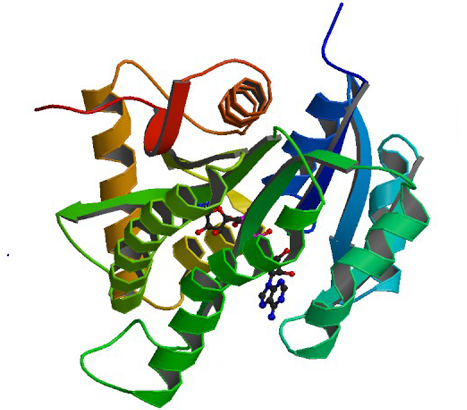
\includegraphics[width=12cm]{images/inha.png}
	\caption{Estrutura 3D em formato de fita da proteína InhA. Imagem obtida em RCSB PDB (www.rcsb.org) do PDB ID 1ENY}
	\label{fig:inha}
\end{figure}

Em sua estrutura, a proteína InhA contém um conjunto de 268 resíduos, que por sua vez são compostos por um total de 4.008 átomos. No PDB (\emph{Protein Data Bank}), a proteína em estudo está identificada pelo código 1ENY.

Conforme descrito em \cite{kar11}, ``A InhA é uma enzima importante no mecanismo de ação da tuberculose pois é responsável pela biossíntese de ácidos graxos, um importante componente da parede celular da micobactéria, e, consequentemente, uma das estruturas essenciais para a sua sobrevivência. Por esse motivo, desperta atenção especial como alvo atraente para o desenvolvimento de novos fármacos para a tuberculose.''

\section{Ligantes Considerados}

O Triclosano (do inglês TCL - \emph{Triclosan}) é um componente químico utilizado para contenção ou prevenção de contaminações bacterianas. É comumente encontrado em produtos domésticos como medicamentos, loções e cremes dentais \cite{TCL}. O TCL está sendo testado como uma alternativa para o desenvolvimento da tuberculose pois age diretamente na inibição do crescimento da bactéria.

De acordo com \cite{GAU08} ``estudos demonstraram que o triclosan também inibe uma enoil-redutase presente em \emph{M. smegmatis} e M. \emph{tuberculosis}. Essa enzima está envolvida com a síntese de ácidos micólicos que são componentes essenciais para a parede celular das  micobactérias e é o principal alvo da INH, um dos mais importantes antimicrobianos utilizados no tratamento da TB.''

A estrutura do TCL consiste em uma pequena molécula composta por um conjunto de 24 átomos. A Figura \ref{fig:tcl} ilustra a estrutura 3D do ligante TCL.

\begin{figure}[h]
	\center
	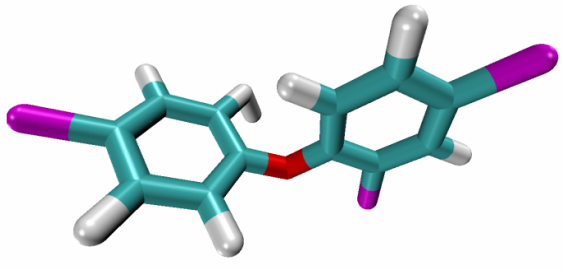
\includegraphics[width=12.5cm]{images/tcl.png}
	\caption{Representação 3D da estrutura do ligante Triclosano \cite{kar11}.}
	\label{fig:tcl}
\end{figure}

Outro ligante empregado nos experimentos de docagem molecular utilizados neste trabalho é o Etionamida (do inglês ETH - \emph{Ethionamide}). O ETH é um antibiótico utilizado no tratamento da tuberculose. É um componente quimico eficaz contra microorganismos do gênero \emph{Mycobacterium}, especialmente as espécies \emph{M. tuberculosis}. 

Conforme descrito em \cite{COH10} ``A ETH se liga covalentemente ao carbono 4 da porção nicotinamida do NADH formando o aduto ETH-NADH, […], este aduto desestabiliza as ligações covalentes que mantêm o NADH em posição no sitio ativo da proteína inibindo a ação da mesma.''

A estrutura do ETH consiste em uma pequena molécula composta por um conjunto de 21 átomos. A Figura \ref{fig:eth} ilustra a estrutura 3D do ligante ETH.

\begin{figure}[h]
	\center
	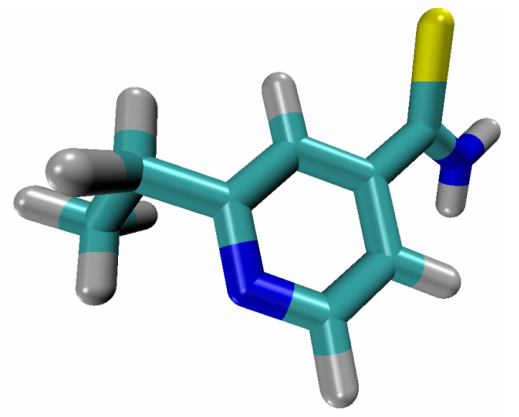
\includegraphics[width=9.5cm]{images/eth.png}
	\caption{Representação 3D da estrutura do ligante Etionamida \cite{kar11}.}
	\label{fig:eth}
\end{figure}

\section{Banco de simulações de docagem}

Primeiramente, os especialistas de domínio do LABIO executaram dois experimentos de docagem molecular, cada um deles envolvendo um ligante diferente. Para o primeiro experimento, foi considerado o TCL como ligante. Já para o segundo, foi utilizado o ligante ETH. Ambos experimentos empregaram a enzima InhA como receptora, e sua flexibilidade foi representada por um conjunto de 3.100 \emph{snapshots} resultantes de simulações por DM. 

Cada ligante foi submetido a 3.100 simulações de docagem, uma para cada conformação do conjunto. Os atributos calculados por estes experimentos foram FEB e RMSD, e após a execução, os dados resultantes dos experimentos foram exportados para um \emph{data set} em formato CSV (\emph{Comma-separated values}).

Neste \emph{data set} os dados estão organizados da seguinte maneira: cada linha representa um dos 3.100 \emph{snapshots} da proteína receptora; nas colunas estão os valores das diferentes posições tridimensionais de cada um dos átomos da proteína e o posicionamento final de cada ligante com seus respectivos valores de FEB e RMSD.

Cada átomo da proteína está representado no \emph{data set} por três colunas, cada uma delas contém respectivamente as coordenadas X, Y e Z de seu posicionamento. As colunas finais apresentam os melhores valores para as métricas FEB e RMSD para cada ligante do experimento. A Tabela \ref{tab:dataset} apresenta a estrutura em que os dados estão organizados no \emph{data set}.

\begin{table}[h]
\caption{Estrutura do \emph{data set} contendo os dados resultantes de experimentos de docagem molecular para os ligantes TCL e ETH.}
\label{tab:dataset}
\scalebox{0.7}{
\begin{tabular}{c|l|l|l|l|l|l|l|l}
\hline
\textbf{SS}   & \multicolumn{1}{c|}{\textbf{ALA\_1\_N\_x}} & \multicolumn{1}{c|}{\textbf{ALA\_1\_N\_y}} & \multicolumn{1}{c|}{\textbf{ALA\_1\_N\_z}} & \multicolumn{1}{c|}{\textbf{...}} & \multicolumn{1}{c|}{\textbf{ETHBESTFEB}} & \multicolumn{1}{c|}{\textbf{ETHBESTRMSD}} & \multicolumn{1}{c|}{\textbf{TCLBESTFEB}} & \multicolumn{1}{c}{\textbf{TCLBESTRMSD}} \\ \hline
\textbf{1}    & 15.834                                     & -20.243                                    & 8.161                                      & ...                               & -8.74                                    & 3.79                                      & -10.52                                   & 5.52                                     \\ \hline
\textbf{2}    & 15.641                                     & -20.046                                    & 8.011                                      & ...                               & -9.34                                    & 3.86                                      & -9.71                                    & 5.77                                     \\ \hline
\textbf{3}    & 15.954                                     & -20.459                                    & 7.796                                      & ...                               & -9.38                                    & 3.60                                      & -9.86                                    & 5.45                                     \\ \hline
\textbf{4}    & 16.321                                     & -20.608                                    & 7.448                                      & ...                               & -9.28                                    & 3.72                                      & -9.23                                    & 5.18                                     \\ \hline
\textbf{...}  & ...                                        & ...                                        & ...                                        & ...                                         & ...                               & ...                                      & ...                                       & ...                                   \\ \hline
\textbf{3100} & 18.591                                     & -17.334                                    & 11.449                                     & ...                               & -9.28                                    & 5.28                                      & 1.25                                     & 7.50                                     \\ \hline
\end{tabular}
}
\end{table} 

Relacionando com o processo de ETL, o \emph{data set} recebido representa uma fonte de dados que deve ser utilizada para extração das informações relevantes para o negócio. Os dados contidos nele não possuem um tratamento, mas foi possível observar uma padronização de nomenclatura das colunas.

%-------------------------------------------------------
% Comandos para os algoritmos:
\renewcommand{\algorithmicfor}{\textbf{para}}
\renewcommand{\algorithmicif}{\textbf{se}}
\renewcommand{\algorithmicthen}{\textbf{então}}
\renewcommand{\algorithmicelse}{\textbf{senão}}
\renewcommand{\algorithmicendif}{\textbf{fim se}}
\renewcommand{\algorithmicendfor}{\textbf{fim para}}
\renewcommand{\algorithmicdo}{\textbf{faça}}
%-------------------------------------------------------

\chapter{Desenvolvimento do modelo OLAP}
\label{cap:DesenvolvimentoDoModeloOLAP}
%-------------------------------------------------------
% descrever como foi feito o levantamento dos residuos mais interesantes. 
%  Explicar que a lista dos mais presentes foi comparada com uma lista originalmente desenvolvida por um especialista de dominio. 
%  Encontrou se casos que estavam e nao estavam na lista, os que nao apareciam na lista constituem de residuos que se ficam ˜proximos”ao sitio de ligação, mas que na realidade estão fora do sítio.
% descrever como  adicionar novas dimensoes baseadas em novos residuos
%-------------------------------------------------------
\section{Levantamento de questões de negócio}
\label{sec:LevantamentoDeQuestoesDeNegocio}

Para possibilitar a construção do modelo OLAP, primeiramente foi necessário identificar e definir as questões de negócio que seriam relevantes sob o ponto de vista do especialista de domínio. Em virtude disso, o levantamento destes dados foi feito por meio de entrevistas com os especialistas do LABIO.

A Tabela \ref{tab:questaoNegocio} descreve as questões de negócio que foram identificadas como sendo mais relevantes para execução de análise de experimentos de docagem realizados no LABIO. 

\begin{table}[h]
\caption{Questões de negócio identificadas pelos especialistas com maior relevância para análise de experimentos de docagem}
\label{tab:questaoNegocio}
\centering
\resizebox{\textwidth}{!}{%
\begin{tabular}{@{}ll@{}}
\toprule
\textbf{ } & \multicolumn{1}{c}{\textbf{Questões de maior relevância para a análise de docagem}}		\\ \midrule
\textbf{1.} & Associar um grupo para cada conformação;													\\
\textbf{2.} & Identificar o comportamento das conformações baseado nas métricas de FEB e RMSD;			\\
\textbf{3.} & Identificar conformações/grupos que possuem o maior número de contatos com os ligantes;	\\
\textbf{4.} & Com base no item 3, identificar quais são os resíduos mais importantes;					\\
\textbf{5.} & Com base no item 3, identificar quais grupos possuem melhores valores de FEB e RMSD.		\\ \bottomrule
\end{tabular}
}
\end{table}

\section{Identificação de métricas}
\label{sec:IdentificacaoDeMetricas}

Durante as entrevistas realizadas, pode-se perceber que informações baseadas nas métricas FEB e RMSD possuíam grande relevância para responder as questões de negócio. Entretanto foi necessário definir certas propriedades e limitações de valores para adequar os cálculos às necessidades do negócio. Dessa maneira, todas as definições citadas nesta seção foram estabelecidas em conjunto com os especialistas de domínio do LABIO, para que os resultados apresentados pudessem representar a realidade.

O cálculo da FEB é um dos métodos utilizados pelos softwares de docagem que permite avaliar a interação receptor-ligante. Quanto menor for o resultado deste cálculo, mais favorável é a ligação estabelecida. Portanto, o valor estimado da FEB é utilizado como uma das métricas do modelo.

Na maioria dos experimentos, os melhores resultados de FEB são valores negativos. Portanto, qualquer conformação que apresente valores de FEB positivos não foram levados em consideração. Dessa maneira evita-se que os resultados positivos venham a interferir em uma análise futura dos valores agregados de um experimento. 

O cálculo do RMSD é utilizado para obter a distância média entre os átomos. Nos experimentos de docagem, este cálculo é feito para comparar o posicionamento inicial do ligante, geralmente estipulada pelo especialista de domínio, com o posicionamento final após a execução da docagem. Neste caso, o RMSD é considerado como uma métrica para a modelagem.

Tanto a FEB quando o RMSD dão uma visão para o especialista de quão satisfatório foi o processo de docagem para uma determinada iteração. Enquanto a FEB mede a qualidade da docagem no aspecto termodinâmico da questão, o RMSD tem como natureza avaliar geometricamente como estão dispostas as moléculas do resíduo e do ligante.

Além disso, para ser possível responder ao item 3 da Tabela \ref{tab:questaoNegocio}, foi necessário incluir uma métrica para contabilizar o número de contatos entre o ligante e um resíduo da molécula receptora. 

Um contato pode ser identificado pelo cálculo da medida em {\AA}ngstr\"om ({\AA}) entre os átomos do resíduo do receptor e do ligante. Ou seja, para cada resíduo do receptor \emph{R} é calculada a distância Euclidiana entre todos seus átomos e os átomos de um ligante \emph{L}. Sendo $R=(r_{x},r_{y},r_{z})$ representando as coordenadas dos átomos dos resíduos do receptor, e $L=(l_{x},l_{y},l_{z})$ representando as coordenadas dos átomos do ligante, o cálculo da distância se dá pela equação \ref{eqt:distEuclid}.

\begin{equation}
\label{eqt:distEuclid}
	d(R,L)=\sqrt{(r_{x}-l_{x})^{2}+(r_{y}-l_{y})^{2}+(r_{z}-l_{z})^{2}}
\end{equation}

Em suma, para cada snapshot devem ser calculadas todas as coordenadas do receptor com todas as coordenadas de cada ligante, neste caso para o TCL e para o ETH. Entretanto, de todas as distâncias calculadas para um resíduo, apenas a menor delas deve ser considerada. 

A Figura \ref{fig:PIFvsGLY} ilustra este conceito, apresentando como exemplo as distâncias entre os átomos do ligante PIF (cor preto) e do resíduo GLY95 (cor cinza) do receptor InhA. Para todas as distâncias calculadas, a menor delas é de 2.72 {\AA} \cite{KARANADUNOSM09}.

\begin{figure}[h]
	\center
	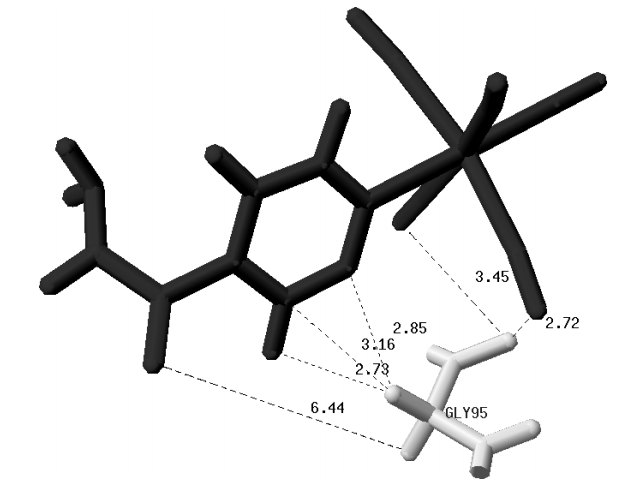
\includegraphics[scale=0.55]{images/distEucli.png}
	\caption{Cálculo das distâncias atômicas entre o ligante PIF (cor preta) e o resíduo GLY95 (cor cinza) do receptor InhA \cite{KARANADUNOSM09}.}
	\label{fig:PIFvsGLY}
\end{figure} 

\section{Definição de relevância para os resíduos}

Um dos pontos mais importantes para responder aos questionamentos dos especialistas de domínio e fundamental para composição das dimensões, consiste em definir os resíduos que são mais relevantes para os experimentos de docagem envolvendo os ligantes TCL e ETH com o receptor InhA. 

A enzima InhA é composta por 268 resíduos, e o processo de identificação dos mais importantes leva em consideração o número de contatos estabelecidos entre os átomos do resíduo e o ligante. No \emph{data set} que foi resultado do processo de simulação de docagem, cada átomo do resíduo está representado por uma tripla, contendo a sua localização espacial nos eixos \emph{x, y }e \emph{z}.

De acordo com o especialista de domínio, a interação entre um átomo do resíduo e o ligante só deve ser considerada como contato quando a distância entre ambos seja entre 2{\AA} e 4{\AA}. Valores inferiores a 2{\AA} são descartados por serem considerados uma sobreposição, enquanto valores superiores a 4{\AA} indicam que não foi estabelecido contato. 

Além disso, uma outra restrição se aplica para os átomos de hidrogênio dos resíduos da molécula receptora. Por apresentarem um comportamento diferente, os átomos de hidrogênio são desconsiderados e não têm suas distâncias calculadas.

Dessa forma, para cada resíduo do receptor deve ser calculada a distância Euclidiana tridimensional de seus átomos utilizando a equação \ref{eqt:distEuclid}, conforme descrito na seção \ref{sec:IdentificacaoDeMetricas}. A partir daí, identifica-se a relevância de um resíduo para o experimento de docagem conforme o número de contatos que são estabelecidos entre seus átomos e o ligante. Quanto mais contatos, mais relevante o resíduo é para o experimento.

As regras de classificação de relevância de um resíduo podem ser sumarizadas da seguinte forma:
\begin{itemize}
	\item Considerar como contatos somente as distâncias entre 2 e 4 {\AA}ngstr\"ons.
	\item Desconsiderar distâncias inferiores a 2 {\AA}ngstr\"ons.
	\item Desconsiderar átomos de hidrogênio.
	\item Quanto maior for o número de contatos estabelecidos de um resíduo, mais relevante ele se torna para o experimento.
\end{itemize}

Assim que foram definidas as limitações e regras de classificação, o esforço foi aplicado na obtenção destes dados. 

Com base em estudos e análises de experimentos anteriores utilizando a InhA como molécula receptora, um especialista de domínio elaborou uma lista dos 52 principais resíduos que possuem relevância para os experimentos de docagem baseados no mesmo cenário. Este artefato foi levado em consideração e serviu como base para identificar os resíduos que fossem relevantes. 

A Tabela \ref{tab:listaOsmar} apresenta a lista elaborada pelo especialista contendo os resíduos representados pela sua sigla e seu número de ordem na enzima.

\begin{table}[h]
\caption{Lista elaborada pelo especialista de domínio com os principais resíduos para experimentos de docagem utilizando a enzima InhA.}
\label{tab:listaOsmar}
\centering
\begin{tabular}{@{}lllllll@{}}
GLY\_13	&	PHE\_40 &	PHE\_96	&	PHE\_148 &	PRO\_191 &	ILE\_201 &	GLU\_209 		\\
ILE\_14	&	LEU\_62 &	MET\_97	&	PRO\_155 &	ILE\_193 &	VAL\_202 &	ALA\_210 		\\
ILE\_15	&	ASP\_63 &	GLN\_99	&	ALA\_156 &	THR\_195 &	GLY\_203 &	ILE\_214 		\\
THR\_16	&	VAL\_64 &	MET\_102 &	TYR\_157 &	LEU\_196 &	GLY\_204 &	LEU\_217 		\\
SER\_18	&	GLN\_65 &	GLY\_103 &	MET\_160 &	ALA\_197 &	ALA\_205 &					\\
SER\_19	&	SER\_93 &	ILE\_121 &	LYS\_164 &	MET\_198 &	LEU\_206 &					\\
ILE\_20	&	ILE\_94	&	MET\_146 &	ALA\_190 &	SER\_199 &	GLY\_207 &					\\
ALA\_21 &	GLY\_95	&	ASP\_147 &	GLY\_191 &	ALA\_200 &	GLU\_208 &					\\ 
\end{tabular}
\end{table}

\section{Identificação dos resíduos relevantes}
\label{sec:IdentificacaoDosResiduosRelevantes}

Durante a fase de desenvolvimento dos scripts necessários para processamento dos dados de docagem e extração das informações relevantes, foi identificada a necessidade de dividir o \emph{data set}. De acordo com os especialistas de domínio, o resíduo NAH deveria ter sua distância euclidiana calculada apenas com o ligante TCL.

Como no \emph{data set} original todas as informações estavam consolidadas em um único arquivo CSV contendo 3.100 linhas e 12.335 colunas, a manipulação destes dados em softwares como o Microsoft Excel se torna praticamente inviável.

Dessa forma, foi desenvolvido um \emph{script} nomeado de ``ajustaColunasDocking'' para fazer a manipulação das colunas do \emph{data set}. O script recebe os seguintes parâmetros de entrada:

\begin{enumerate}
	\item Sinal da operação a ser feita (`-m' mantém as colunas, e `-e' remove as colunas);
	\item Nome das colunas que serão manipuladas separadas por vírgula;
	\item Arquivo de entrada com dados de docagem (\emph{data set});
	\item Arquivo de saída com as colunas manipuladas.
\end{enumerate}

O Algoritmo \ref{alg:ajustaColunaDocking} descreve o processo de funcionamento do script ``ajustaColunasDocking''.

\floatname{algorithm}{Algoritmo}
\begin{algorithm}[H]
\caption{Algoritmo para manipulação da base de dados da simulação de docagem molecular}
\label{alg:ajustaColunaDocking}
{\fontsize{10}{10}\selectfont
\begin{algorithmic}[1]
	\STATE Seja C a lista com o nome das colunas
	\STATE Seja D a base de dados dos resultados da simulação de docagem molecular
	\STATE Seja c uma coluna em C
	\STATE Seja d uma linha em D
	\STATE Seja M o modo de operação da execução
	\IF{M for igual a manter as colunas em C}
		\FOR{cada d em D}
			\FOR{cada c em C}
			\STATE Grave apenas c na saída
			\ENDFOR
		\ENDFOR
	\ENDIF
	\IF{M for igual a excluir as colunas em C}
		\FOR{cada d em D}
			\FOR{cada c em C}
			\STATE Remove apenas c na saída
			\ENDFOR
		\ENDFOR
	\ENDIF
\end{algorithmic}
}
\end{algorithm}

O algoritmo ``ajustaColunasDocking'' foi utilizado para remover os dados referentes aos átomos do resíduo NAH do \emph{data set} original e separá-los em outro arquivo de dados distinto. Após a manipulação, os arquivos de dados ficaram da seguinte forma:
\begin{itemize}
	\item \emph{Data set} 1: Removidas todas as colunas dos átomos referentes ao resíduo NAH.
	\item \emph{Data set} 2: Apenas dados dos átomos referentes ao resíduo NAH e do ligante TCL.
\end{itemize}

Neste ponto é importante ressaltar que ambos os arquivos tiveram somente suas colunas alteradas e mantiveram um total de 3.100 linhas, representando a trajetória das conformações da molécula receptora.

Com os arquivos devidamente separados de acordo com os critérios estabelecidos, foi possível realizar o cálculo da distância Euclidiana. Para isso, foi desenvolvido um segundo \emph{script}, nomeado ``calculaDistancia'', que realiza o cálculo de todo o conjunto de átomos existente em um \emph{data set} tendo como base os critérios definidos previamente para classificação da relevância dos resíduos.

Para execução do \emph{script} ``calculaDistancia'', são necessários três parâmetros de entrada, sendo eles:
\begin{enumerate}
	\item Arquivo contendo lista de átomos do resíduo da molécula;
	\item Arquivo contendo lista de átomos do(s) ligante(s);
	\item Arquivo de entrada com dados de docagem (\emph{data set}).
\end{enumerate}

%-----------------------------------
% 
%    TO DO: verificar as informações de saída do script
%
%       
%-----------------------------------

A partir dos três arquivos de entrada é gerado um arquivo de saída em formato CSV contendo as seguintes informações: número do \emph{snapshot}, nome do resíduo, nome do ligante, resultado do cálculo da distância, classificação da distância (se foi menor que 2 ou está entre 2 e 4 {\AA}ngstr\"ons).
O Algoritmo \ref{alg:CalculoDistancia} descreve o processo de funcionamento do \emph{script} "calculaDistancia.

\floatname{algorithm}{Algoritmo}
\begin{algorithm}[H]
\caption{Algoritmo para cálculo da distância}
\label{alg:CalculoDistancia}
{\fontsize{10}{10}\selectfont
\begin{algorithmic}[1]
	\STATE Seja R uma lista composta por resíduos e seus átomos
	\STATE Seja L uma lista de ligantes
	\STATE Seja D a base de dados dos resultados da simulação de docagem molecular
	\STATE Seja r uma tupla com a posição x, y e z de um resíduo juntamente com seu átomo em R
	\STATE Seja l um ligante de L
	\STATE Seja d um \emph{snapshot} da conformação da base D
	\FOR{cada d em D}
		\FOR{cada r em R}
			\FOR{cada l em L faça}
			\IF{r não conter átomo de hidrogênio}
			\STATE Distância $\gets \sqrt{(rx - lx)^{2} +(ry - ly)^{2} + (rz - lz)^{2}}$ 
			\ENDIF
			\IF{Distância menor que 4}
				\IF{Distância menor ou igual a 2}
				\STATE Gravar na saída d, r, l, distancia, classificação menor que 2
				\ELSE
				\STATE Gravar na saída d, r, l, distancia, classificação entre 2 e 4
				\ENDIF
			\ENDIF
			\ENDFOR
		\ENDFOR
	\ENDFOR
\end{algorithmic}
}
\end{algorithm}

%-----------------------------------
% 
%    TO DO: colocar screenshot do output do script
%
%       
%-----------------------------------

Após a execução do algoritmo para calcular as distâncias os dados de saída foram sumarizados. Como resultado, foi obtida uma listagem de 15 resíduos com maior número de contatos comuns para os experimentos de docagem envolvendo ambos ligantes TCL e ETH. A Tabela \ref{tab:listaProvavelRelevantes} lista os resíduos obtidos pelo algoritmo, que estão representados pela sua sigla e seu número de ordem na enzima.

\begin{table}[h]
	\caption{Resíduos identificados pelo algoritmo de cálculo.}
	\label{tab:listaProvavelRelevantes}
	\centering
	\begin{tabular}{@{}lll@{}}
	ILE\_15  & ASP\_149 & MET\_160 \\
	SER\_19  & ARG\_152 & ILE\_193 \\
	ILE\_94  & ALA\_153 & THR\_195 \\
	GLY\_95  & MET\_154 & MET\_198 \\
	PHE\_148 & TYR\_157 & TRP\_221 \\
	\end{tabular}
\end{table}

Com posse destes dados, os resíduos resultantes (apresentados na Tabela \ref{tab:listaProvavelRelevantes}) foram comparados com a lista feita pelo especialista de domínio (apresentados na Tabela \ref{tab:listaOsmar}) a fim de identificar os elementos que eram comuns aos dois grupos. 

Dos 15 resíduos identificados pelo algoritmo, 10 deles estão presentes na lista do especialista de domínio e foram classificados como sendo relevantes para os experimentos de docagem. Os 5 resíduos que não estavam presentes na lista do especialista foram identificados como casos onde a proteína apresentou ligações fora da cavidade do substrato e, por este motivo, não foram considerados como sendo relevantes. Os resíduos do conjunto obtido foram plotados pelos especialistas de domínio do LABIO e estão ilustrados pela Figura \ref{fig:PlotResiduos}. 

\begin{figure}[h]
        \center
        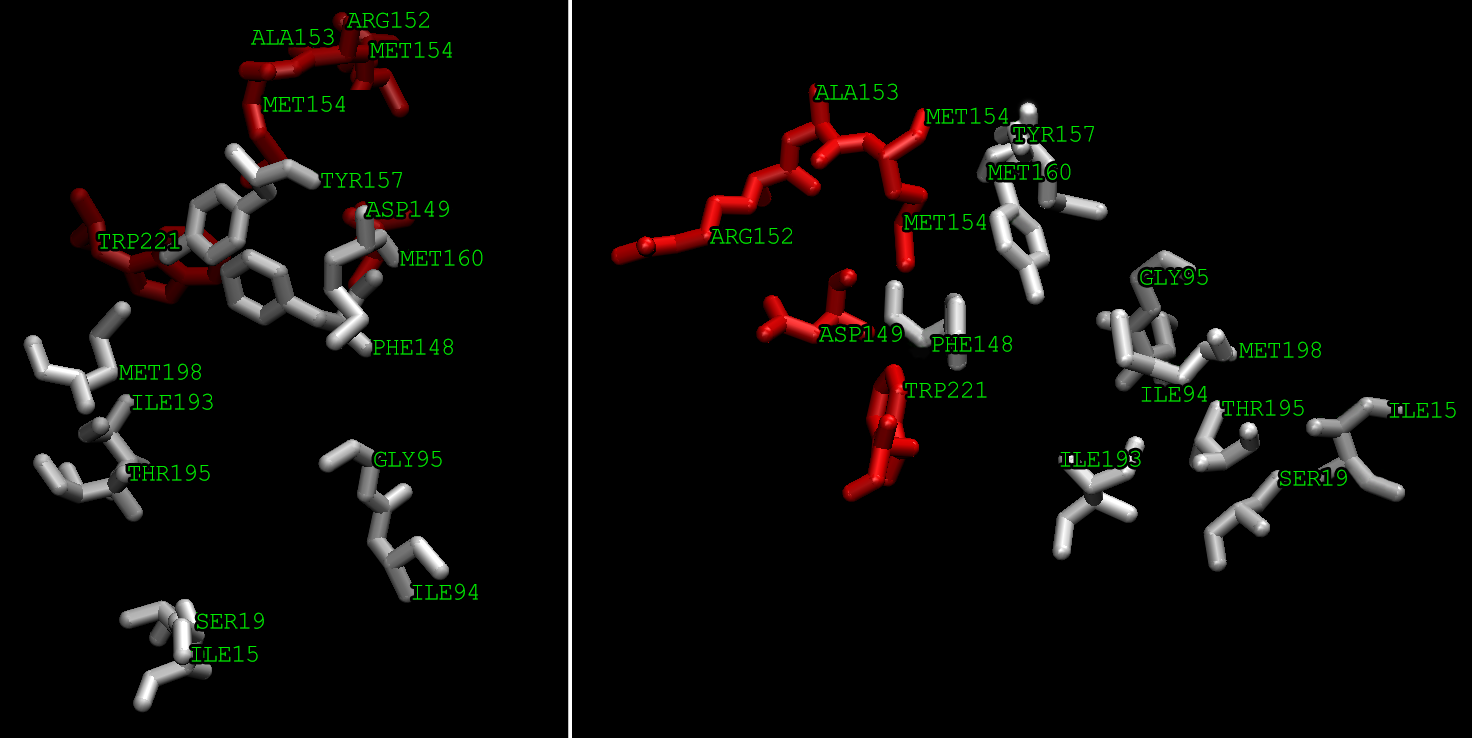
\includegraphics[scale=0.55]{images/avaliacao_Residuos_nomes.png}
        \label{fig:PlotResiduos}
        \caption{Plotagem dos 15 resíduos identificados pelo algoritmo de classificação por relevância. A cor cinza representa os resíduos que são relevantes e aparecem na listagem do especialista de domínio, já os resíduos que estão em vermelho não estão presentes na lista.}
\end{figure}

Com base nos algoritmos executados e nas comparações realizadas, foi possível elencar os 10 principais resíduos mais relevantes para responder às questões de negócio. O conjunto final está listado na Tabela \ref{tab:listaProvavelRelevantes}, a qual foi utilizada como base para a modelagem OLAP.

\begin{table}[h]
\caption{Conjunto final de resíduos relevantes para experimentos de docagem molecular considerando como receptor a enzima da InhA e ligantes TCL e ETH.}
\label{tab:listaProvavelRelevantes}
\centering
\begin{tabular}{@{}ll@{}}
\toprule
\textbf{Resíduo} 		    & \textbf{Nome} 		 \\ \midrule
SER\_19                     & Serina                   \\
ILE\_15                     & Isoleucina               \\
ILE\_94                     & Isoleucina               \\
GLY\_95                     & Glicina                  \\
PHE\_148                    & Fenilalanina             \\
TYR\_157                    & Tirosina                 \\
MET\_160                    & Metionina                \\
ILE\_193                    & Isoleucina               \\
THR\_195                    & Treonina                 \\
MET\_198                    & Metionina                \\ \bottomrule
\end{tabular}
\end{table}

\section{Modelagem da solução}
\label{sec:ModelagemDaSolucao}

Para atender às questões de negócio levantadas pelos especialistas de domínio conforme descrito na Tabela \ref{tab:questaoNegocio}, foi proposto um modelo de dados do tipo estrela contendo uma tabela fato e quinze dimensões. 

A modelagem proposta foi baseada na resolução das questões de negócio específicas para o cenário descrito neste trabalho, porém este mesmo modelo pode ser empregado em outros tipos de experimentos. A Figura \ref{fig:ConcepcaoModeloOLAP} ilustra o projeto inicial da modelagem OLAP.

\begin{figure}[h]
        \center
        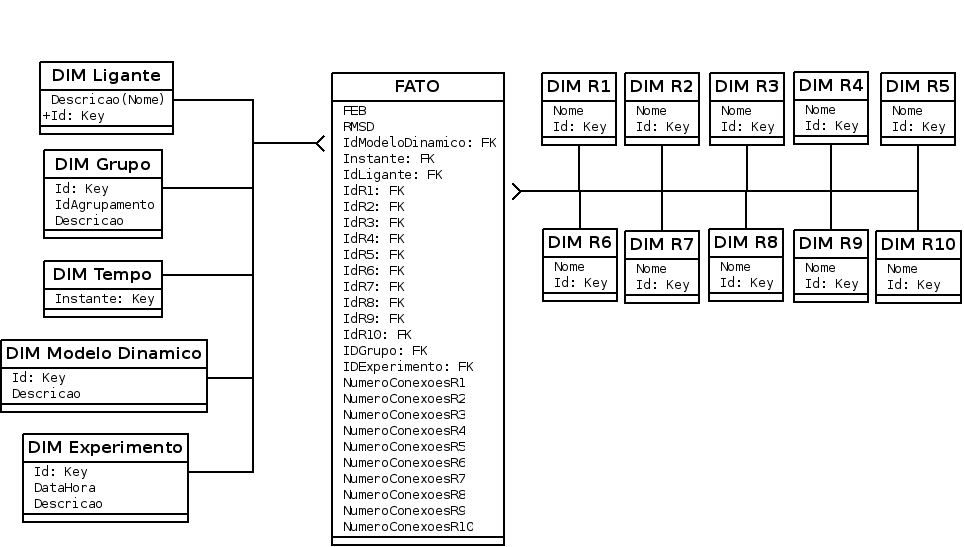
\includegraphics[scale=0.45]{images/Modelo_OLAP.png}
        \caption{Concepção inicial do modelo OLAP}
        \label{fig:ConcepcaoModeloOLAP}
\end{figure}

A tabela fato foi projetada tendo como base as métricas identificadas na Seção \ref{sec:IdentificacaoDeMetricas}, ou seja: FEB, RMSD e número de contatos. As métricas de FEB e RMSD foram representadas na tabela fato pelos atributos ``FEBMedio'' e ``RMSDMedio'', ambos utilizando o cálculo de valor médio.

Como foi elencado um conjunto contendo 10 resíduos mais importantes para o experimento, a métrica de número de contatos deve valer para cada um dos resíduos, apresentando o número de ligações entre o resíduo e o ligante. Para representar isso na fato, foram criadas as métricas \emph{``NumeroConexoesR1'', ``NumeroConexoesR2'', ..., ``NumeroConexoesR10''}, estes realizando apenas o cálculo de somatório. Já as dimensões para os resíduos, foram representadas por ``DIM\_R1'' até ``DIM\_R10''.

A dimensão ``DIM\_Ligante'' representa os ligantes utilizados no experimento, neste caso o TCL e ETH.

O conjunto de conformações utilizado é de 3.100 conformações, a qual representa a trajetória dinâmica da molecula durante 3.100 picosegundos (ps). Neste cas o número da conformação se equivale ao instante de tempo, por exemplo, o snapshot 500 refere-se a conformação da molécula receptorna no instante de 500ps. Com isso, o tempo foi representado pela dimensão ``DIM\_Tempo''. 

A dimensão ``DIM\_Modelo\_Dinamico'' serve para o especialista de domínio identificar qual foi a dinâmica utilizada no experimento. No caso deste trabalho, foi utilizada apenas uma dinâmica de 3.100 conformações.

Um experimento de docagem utiliza agrupamentos para determinadas conformações, com base na semelhança existente entre elas. Dessa forma, foi necessário permitir a que estes agrupamentos fossem identificados, para possibilitar a análise por agrupamento. Esta necessidade foi representada pela dimensão ``DIM\_Grupo''.

Por fim, a dimensão ``DIM\_Experimento'' serve para o especialista de domínio identificar as informações relacionadas ao experimento executado. Um mesmo experimento de docagem poder ser executado mais de uma vez utilizando modelos dinâmicos diferentes. Com esta dimensão os experimentos são separados com base nas informações providas pelo especialista de domínio.


\section{Construção do modelo no Analisys Services}

A modelagem inicial do OLAP se mostrou apto para responder as questões de negócio que foram levantadas no início do projeto. Com isso, modelo foi construído utilizando as ferramentas Microsoft Analysys Services e o banco de dados Microsoft SQL Server. A Figura \ref{fig:ModeloOLAP} ilustra o modelo já criado no Analysis Services.

\begin{figure}[h]
        \center
        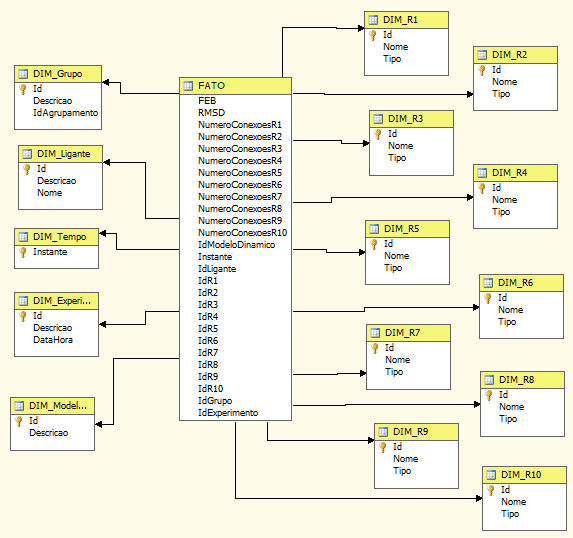
\includegraphics[scale=1]{images/ModelagemOLAP.PNG}
        \caption{Modelo OLAP construído com uso do Microsoft Analysis Services.}
        \label{fig:ModeloOLAP}
\end{figure}

A seguir descrevem-se todas as definições e propriedades levadas em consideração durante a criação do modelo OLAP no Analysis Services, bem como a definição de cada campo:
	
\begin{itemize}
	\item
		\textbf{Tabela:} DIM\_Grupo \\
		\textbf{Tipo:} Dimensional. \\
		\textbf{Descrição:} Representa os agrupamentos de conformações por semelhança.
\end{itemize}
\begin{table}[h]
	\caption{Dimensão DIM\_Grupo}
	\centering
	\begin{tabular}{@{}llll@{}}
	\toprule
	\textbf{Nome} & \textbf{Tipo} & \textbf{PK} & \textbf{Descrição}           		\\ \midrule
	Id            & Numeric           & x           & Identificador da dimensão grupo   \\
	Descricao     & Char       &             & Descrição do grupo           		\\
	IdAgrupamento & Numeric          &             & Identificador do agrupamento 		\\ \bottomrule
	\end{tabular}
\end{table}

% \begin{figure}[h]
%         \center
%         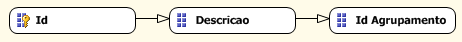
\includegraphics[scale=1]{images/A_DIM_Grupo.PNG}
%         \caption{Hierarquia da dimensão DIM\_Grupo}
%         \label{fig:ModeloOLAP}
% \end{figure}

\newpage

\begin{itemize}
	\item
		\textbf{Tabela:} Fato \\
		\textbf{Tipo:} Fato. \\
		\textbf{Descrição:} Representa todos os eventos de um experimento.
\end{itemize}
\begin{table}[!htbp]
	\caption{Tabela Fato}
	\centering
	\begin{tabular}{@{}llll@{}}
	\toprule
	\textbf{Nome} & \textbf{Tipo} & \textbf{FK} & \textbf{Descrição}           				\\ \midrule
	FEB            			 & Numeric        &             & Valor médio de FEB			    \\
	RMSD    				 & Numeric        &             & Valor médio de RMSD          		\\
	NumeroConexoesR1 	     & Numeric        &             & Numero de ligações do resíduo 1   \\
	NumeroConexoesR2 	     & Numeric        &             & Numero de ligações do resíduo 2   \\
	NumeroConexoesR3 	     & Numeric        &             & Numero de ligações do resíduo 3   \\
	NumeroConexoesR4 	     & Numeric        &             & Numero de ligações do resíduo 4   \\
	NumeroConexoesR5 	     & Numeric        &             & Numero de ligações do resíduo 5   \\
	NumeroConexoesR6 	     & Numeric        &             & Numero de ligações do resíduo 6   \\
	NumeroConexoesR7 	     & Numeric        &             & Numero de ligações do resíduo 7   \\
	NumeroConexoesR8 	     & Numeric        &             & Numero de ligações do resíduo 8   \\
	NumeroConexoesR9 	     & Numeric        &             & Numero de ligações do resíduo 9   \\
	NumeroConexoesR10 	     & Numeric        &             & Numero de ligações do resíduo 10  \\
	Instante 	    		 & Numeric        &  x          & Identificador do instante de tempo  \\
	IdLigante 	    		 & Numeric        &  x          & Identificador do Ligante 			\\
	IdR1 				     & Numeric        &  x          & Identificador do resíduo 1   	\\
	IdR2 				     & Numeric        &  x          & Identificador do resíduo 2   	\\
	IdR3 				     & Numeric        &  x          & Identificador do resíduo 3   	\\
	IdR4 				     & Numeric        &  x          & Identificador do resíduo 4   	\\
	IdR5 				     & Numeric        &  x          & Identificador do resíduo 5   	\\
	IdR6 				     & Numeric        &  x          & Identificador do resíduo 6   	\\
	IdR7 				     & Numeric        &  x          & Identificador do resíduo 7   	\\
	IdR8 				     & Numeric        &  x          & Identificador do resíduo 8   	\\
	IdR9 				     & Numeric        &  x          & Identificador do resíduo 9   	\\
	IdR10			 	     & Numeric        &  x          & Identificador do resíduo 10  	\\	
	IdGrupo			 	     & Numeric        &  x          & Identificador do grupo  		\\	
	IdExperimento 			 & Numeric        &  x          & Identificador do experimento 	\\ \bottomrule
	\end{tabular}
\end{table}

\begin{itemize}
	\item
		\textbf{Tabela:} DIM\_Tempo \\
		\textbf{Tipo:} Dimensional. \\
		\textbf{Descrição:} Representa o tempo em picosegundo. \\
\end{itemize}
\begin{table}[h]
	\caption{Dimensão DIM\_Tempo}
	\centering
	\begin{tabular}{@{}llll@{}}
	\toprule
	\textbf{Nome} 	& \textbf{Tipo} & \textbf{PK} & \textbf{Descrição}           		\\ \midrule			
	Instante 		& Numeric 	       &  x           & Instante de tempo 					\\ \bottomrule
	\end{tabular}
\end{table}

\begin{itemize}
	\item
		\textbf{Tabela:} DIM\_Ligante \\
		\textbf{Tipo:} Dimensional. \\
		\textbf{Descrição:} Representa o ligante utilizado no experimento. \\
\end{itemize}
\begin{table}[h]
	\caption{Dimensão DIM\_Ligante}
	\centering
	\begin{tabular}{@{}llll@{}}
	\toprule
	\textbf{Nome} & \textbf{Tipo} & \textbf{PK} & \textbf{Descrição}           		   \\ \midrule
	Id            & Numeric           & x           & Identificador da dimensão ligante    \\
	Descricao     & Char      &             & Descrição do ligante           	   \\
	Nome 		  & Char       &             & Nome do ligante 					   \\ \bottomrule
	\end{tabular}
\end{table}

% \begin{figure}[h]
%         \center
%         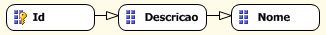
\includegraphics[scale=1]{images/A_DIM_Ligante.PNG}
%         \caption{Hierarquia da dimensão DIM\_Ligante}
%         \label{fig:ModeloOLAP}
% \end{figure}

\begin{itemize}
	\item
		\textbf{Tabela:} DIM\_Experimento \\
		\textbf{Tipo:} Dimensional. \\
		\textbf{Descrição:} Representa o tipo do experimento executado. \\
\end{itemize}

\begin{table}[h]
	\caption{Dimensão DIM\_Experimento}
	\centering
	\begin{tabular}{@{}llll@{}}
	\toprule
	\textbf{Nome} 	& \textbf{Tipo} & \textbf{PK} & \textbf{Descrição}           			\\ \midrule
	Id            	& Numeric           & x           & Identificador da dimensão experimento   \\
	Descricao     	& Char       &             & Descrição do tipo de experimento        \\
	DataHora 		& Date 		    &             & Data e hora do experimento executado 	\\ \bottomrule
	\end{tabular}
\end{table}

% \begin{figure}[h]
%         \center
%         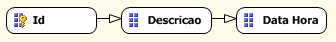
\includegraphics[scale=1]{images/A_DIM_Experimento.PNG}
%         \caption{Hierarquia da dimensão DIM\_Experimento}
%         \label{fig:ModeloOLAP}
% \end{figure}

\begin{itemize}
	\item
		\textbf{Tabela:} DIM\_Modelo\_Dinamico \\
		\textbf{Tipo:} Dimensional. \\
		\textbf{Descrição:} Representa qual dinâmica utilizada no experimento. \\
\end{itemize}
\begin{table}[!htbp]
	\caption{Dimensão DIM\_Modelo\_Dinamico}
	\centering
	\begin{tabular}{@{}llll@{}}
	\toprule
	\textbf{Nome} 	& \textbf{Tipo} & \textbf{PK} & \textbf{Descrição}           			\\ \midrule
	Id            	& Numeric           & x           & Identificador da dimensão modelo dinamico   \\
	Descricao     	& Char       &             & Descrição da dinamica utilizada        \\ \bottomrule
	\end{tabular}
\end{table}

% \begin{figure}[h]
%         \center
%         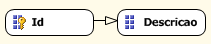
\includegraphics[scale=1]{images/A_DIM_Modelo_Dinamico.PNG}
%         \caption{Hierarquia da dimensão DIM\_Modelo\_Dinamico}
%         \label{fig:ModeloOLAP}
% \end{figure}

\begin{itemize}
	\item
		\textbf{Tabelas:} DIM\_R1 a DIM\_R10 \\
		\textbf{Tipo:} Dimensional. \\
		\textbf{Descrição:} Representa um dos dez principais resíduos para o experimento. \\
\end{itemize}
\begin{table}[!htbp]
	\caption{Dimensões DIM\_R1 a DIM\_R10}
	\centering
	\begin{tabular}{@{}llll@{}}
	\toprule
	\textbf{Nome} 	& \textbf{Tipo} & \textbf{PK} & \textbf{Descrição}           		\\ \midrule
	Id            	& Numeric           & x           & Identificador da dimensão residuo   \\
	Nome 		  & Char       &             & Nome do residuo 					   	\\ 
	Tipo          & Char       &             & Tipo do residuo           	   		\\ \bottomrule   
	\end{tabular}
\end{table}
	
\newpage

A Figura \ref{fig:hierarGrupoLiganteExperimentoModelo} apresenta a composição das hierarquias para as dimensões DIM\_Grupo, DIM\_Experimento, DIM\_Ligante e DIM\_Modelo\_Dinamico respectivamente. Já a Figura \ref{fig:HierarR1ateR10} apresenta a hierarquia para as dimensões dos resíduos de 1 à 10.

\begin{figure}[h]
        \center
        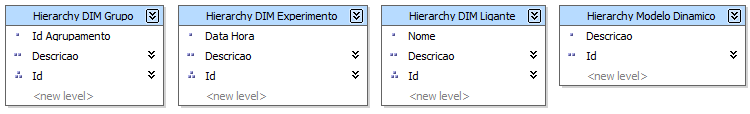
\includegraphics[scale=0.6]{images/Hierar_Grupo_Ligante_Experimento_Modelo.png}
        \caption{Hierarquias das dimensões Grupo, Ligante, Experimento e Modelo Dinâmico}
        \label{fig:hierarGrupoLiganteExperimentoModelo}
\end{figure}

\begin{figure}[h]
        \center
        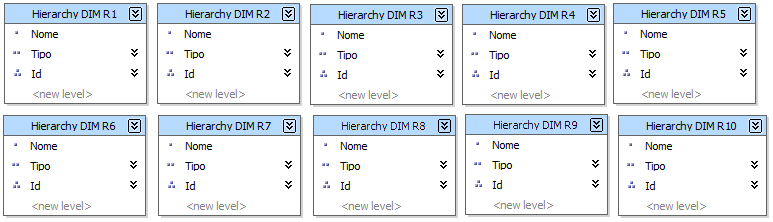
\includegraphics[scale=0.6]{images/Hierar_DIMR1_ate_10.png}
        \caption{Hierarquia das dimensões R1, R2, R3, R4, R5, R6, R7, R8, R9 e R10}
        \label{fig:HierarR1ateR10}
\end{figure}	

\section{Carga de dados no Analysis Services}
\label{sec:CargaDeDadosNoAnalysisServices}

Para o processo de carga dos dados foram desenvolvidos dois scripts e consiste na execução de ambos. O primeiro deles nomeado como ``criaDadosDIMTempo'' tem como objetivo fornecer um \emph{script} SQL para inserção dos dados para a dimensão tempo. O \emph{script} ``criaDadosDIMTempo'' recebe apenas um parâmetro de entrada para execução que é o número de picosegundos que vão ser populados na tabela do banco de dados. A saída é um comando de \emph{INSERT} em SQL para gravação na base de dados, obedecendo a limitação do \emph{SQL Server} de 1000 linhas para cada inserção de múltiplas linhas. O Algoritmo \ref{alg:criaDadosDIMTempo} descreve o funcionamento do \emph{script} ``criaDadosDIMTempo''. 

\floatname{algorithm}{Algoritmo}
\begin{algorithm}[H]
\caption{Algoritmo para popular os dados na dimensão tempo}
\label{alg:criaDadosDIMTempo}
{\fontsize{10}{10}\selectfont
\begin{algorithmic}[1]
	\STATE Seja P um valor inteiro maior que 1
	\STATE Seja L uma lista de valores
	\STATE Seja c um contador
	\FOR{iteração em P}
		\STATE Incrementa mais um em c
		\IF{c igual a 1000}
			\STATE Armazena o valor de P em L
			\STATE Grave o comando de inserção baseado em L
			\STATE Esvazie L
			\STATE Atribua zero em c
		\ELSE
			\STATE Armazena valor de P em L
		\ENDIF
	\ENDFOR
	\IF{L não estiver vazia}
		\STATE Grave o comando de inserção baseado em L
	\ENDIF
\end{algorithmic}
}
\end{algorithm}

O segundo \emph{script} desenvolvido, nomeado de ``criaDados'' é responsável por extrair e realizar a carga de todo o restante das informações contidas no \emph{data set} para a base de dados. Para sua execução são necessários 8 parâmetros de entrada, sendo 4 deles referentes às dimensões que serão populadas, e os outros 4 são arquivos distintos gerados pelos scripts executados previamente.

Os parâmetros de entrada para execução do script ``criaDados'' são os seguintes:
\begin{enumerate}
	\item CSV de entrada contendo os campos da dimensão DIM\_Grupo;
	\item CSV de entrada contendo os campos da dimensão DIM\_Ligante;
	\item CSV de entrada contendo os campos da dimensão DIM\_Experimento;
	\item CSV de entrada contendo os campos da dimensão DIM\_Modelo\_Dinamico;
	\item Arquivo de entrada contendo a lista dos resíduos relevantes;
	\item Arquivo de entrada contendo a relação de contatos por resíduo (gerado pelo Algoritmo \ref{alg:CalculoDistancia});
	\item Arquivo de entrada com dados de docagem (\emph{data set});
	\item Arquivo de entrada com o agrupamento das conformações;
\end{enumerate}

Por fim, após a execução completa do \emph{script}, é gerado os comandos de \emph{INSERT} em SQL para popular as informações no banco de dados. O Algoritmo \ref{alg:criaDadosFato} descreve o funcionamento do \emph{script} ``criaDados''.

\floatname{algorithm}{Algoritmo}
\begin{algorithm}[H]
\caption{Algoritmo para popular os dados na fato}
\label{alg:criaDadosFato}
{\fontsize{10}{10}\selectfont
\begin{algorithmic}[1]
	\STATE Seja L uma lista de ligantes
	\STATE Seja l um ligante em L
	\STATE Seja G uma lista de grupos
	\STATE Seja g um grupo em G
	\STATE Seja M uma lista de modelos dinâmicos
	\STATE Seja m um modelo dinâmico em M
	\STATE Seja E uma lista de experimentos
	\STATE Seja e um experimento em E
	\STATE Seja R uma lista de resíduos mais importantes
	\STATE Seja r um resíduo em R
	\STATE Seja S uma lista de numero de contato dos resíduos
	\STATE Seja s o numero de um contato em S
	\STATE Seja D a base de dados dos resultados da simulação de docagem molecular
	\STATE Seja d uma conformação em D
	\STATE Seja a um agrupamento de d
	\STATE Seja C uma lista de comandos para inserção
	\FOR{cada l em L}
		\STATE Grave o comando de inserção baseado em l
	\ENDFOR
        \FOR{cada g em G}
		\STATE Grave o comando de inserção baseado em g
        \ENDFOR
        \FOR{cada m em M}
		\STATE Grave o comando de inserção baseado em m
        \ENDFOR
        \FOR{cada e em E}
		\STATE Grave o comando de inserção baseado em e
        \ENDFOR
	\FOR{cada r em R}
		\STATE Grave o comando de inserção baseado em r
	\ENDFOR
	\FOR{cada d em D}
		\STATE Grave a em C
		\FOR{cada l em L}
			\FOR{cada s em S}
				\STATE Gravar o valor de s em C para a composição baseando em d, l e r
			\ENDFOR
			\IF{FEB de d for positiva}
				\STATE Gravar 0 para FEB de d em C
			\ELSE
				\STATE Gravar FEB de d em C
			\ENDIF
			\STATE Gravar RMSD de d em C
			\STATE Gravar o comando de inserção baseado em C
		\ENDFOR
	\ENDFOR
\end{algorithmic}
}
\end{algorithm}

Em suma, os scripts desenvolvidos para auxiliar no processo de ETL utilizados durante este trabalho foram executados na seguinte sequência:
\begin{enumerate}
    \item Execução do \emph{script} ``ajustaColunasDocking'' - Separar o resíduo NAH e cria um \emph{data set} auxiliar.
    \item Execução do \emph{script} ``calculaDistancia'' - Calcular distância Euclidiana par os dois \emph{data sets}.
    \item Execução do \emph{script} ``criaDadosDIMTempo'' - Popular a dimensão tempo no banco de dados.
    \item Execução do \emph{script} ``criaDados'' - Popular o restante das informações no banco de dados.
\end{enumerate}



\chapter{Resultados Obtidos}

Conforme visto no capítulo 5 através da tabela \ref{tab:questaoNegocio}, foram elencadas 5 questões que os especialistas de domínio entenderam ser necessárias. A partir do desenvolvimento do modelo OLAP, detalhado na primeira seção do capítulo 5, e dos processos de carga através dos \emph{scripts} de ETL elaborados dentro do trabalho, foi possível a criação do cubo e suas respectivas dimensões dentro do \emph{Microsoft Analysis Services}. Durante o período de criação das dimensões e do próprio cubo, foram realizadas reuniões com os especialistas para adequar o modelo OLAP de maneira que fosse possível endereçar todos os pontos levantados. 

Após a primeira execução e exibição dos resultados no cubo, os especialistas observaram que a FEB média para o ligante Triclosano estava positiva. Inicialmente acreditou-se que era um problema da carga mas, depois de avaliar os resultados da docagem diretamente na base de dados das conformações, viu-se que boa parte dos resultados da melhor FEB para o ligante Triclosano era realmente positivo. Os especialistas então pediram que todo e qualquer FEB positivo fosse substituído pelo valor 0, conforme descrito na seção \ref{sec:IdentificacaoDeMetricas}. Com esta alteração foi necessário realizar uma nova carga dos dados.

Para exibir os resultados e para realizar a composição dos valores e dimensões afim de responder às questões de negócio, foi utilizado o \emph{plug-in} do \emph{Microsoft Excel} para o \emph{Analysis Services}. A figura \ref{fig:questao1} mostra a associação dos agrupamentos para cada uma das conformações, respondendo assim a primeira questão. 

\begin{figure}[h]
        \center
        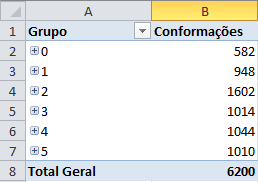
\includegraphics[width=14cm]{images/Questao1.PNG}
        \caption{Resultado para a primeira questão}
        \label{fig:questao1}
\end{figure}

A figura \ref{fig:questao2} exibe o comportamento de cada agrupamento das conformações, levando em consideração a FEB e RMSD médios, respondendo assim a segunda questão levantada pelos especialistas de domínio.

\begin{figure}[h]
        \center
        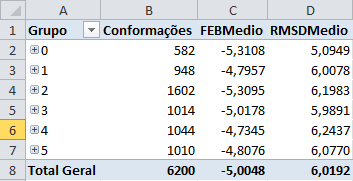
\includegraphics[width=14cm]{images/Questao2.PNG}
        \caption{Resultado para a segunda questão}
        \label{fig:questao2}
\end{figure}

A figura \ref{fig:questao3} mostra os agrupamentos das conformações por cada número de contato dos resíduos com o ligante, possibilitando levantar qual ou quais possuem maior número de contatos estabelecidos e desta forma respondendo a terceira questão de negócio. 

\begin{figure}[h]
        \center
        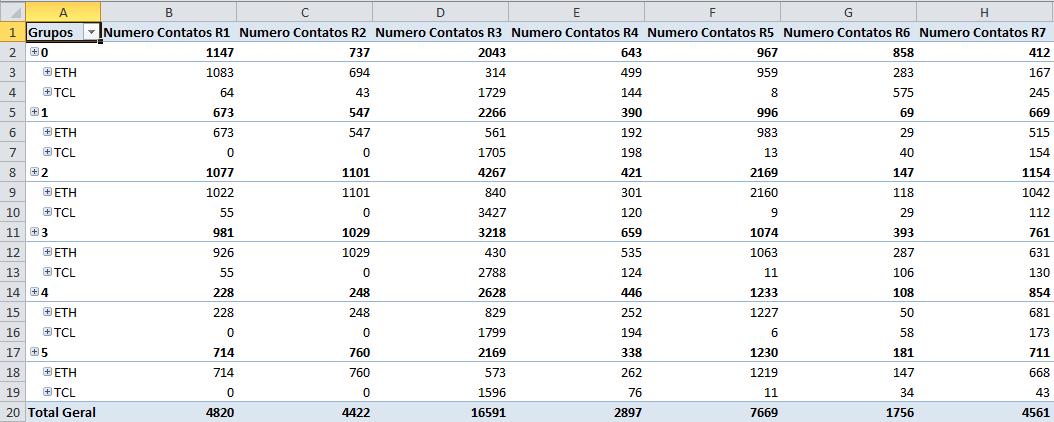
\includegraphics[width=14cm]{images/Questao3.PNG}
        \caption{Resultado para a terceira questão}
        \label{fig:questao3}
\end{figure}

A figura \ref{fig:questao4} mostra qual foi o número de contatos de cada um dos principais resíduos em relação aos agrupamentos das conformações. Esta composição permite identificar quais são os resíduos mais importantes por agrupamento, respondendo assim a quarta questão da tabela \ref{tab:questaoNegocio}.

\begin{figure}[h]
        \center
        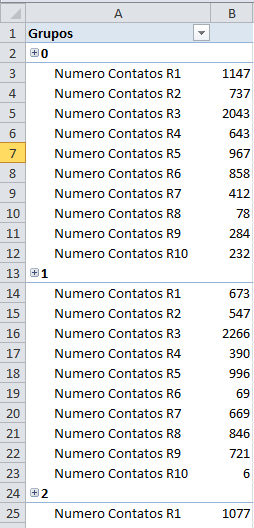
\includegraphics[width=14cm]{images/Questao4.PNG}
        \caption{Resultado para a quarta questão}
        \label{fig:questao4}

Para a quinta e última questão, a figura \ref{fig:questao5} exibe qual foi o FEB e RMSD médios para cada um dos agrupamentos, permitindo avaliar quais grupos possuem os melhores resultados para estas métricas.

\end{figure}\begin{figure}[h]
        \center
        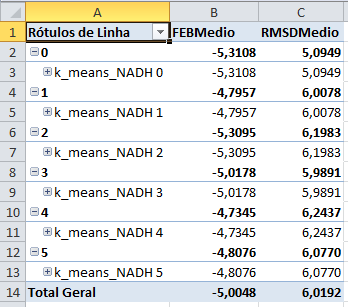
\includegraphics[width=14cm]{images/Questao5.PNG}
        \caption{Resultado para a quinta questão}
        \label{fig:questao5}
\end{figure}

\chapter{Conclusão}

O uso de um modelo OLAP para análise de dados de experimentos de simulações de docagem molecular é uma abordagem nova. Apesar do conjunto de dados utilizados para o desenvolvimento deste trabalho ter sido relativamente pequeno, contendo apenas 3.100 conformações para cada um dos dois ligantes, o modelo OLAP construído se mostrou eficiente para analisar os dados através de uma perspectiva multidimensional.

Certamente com o uso contínuo desta solução, por um maior período de tempo e utilizando uma exaustiva massa de informações de experimentos de docagem, o modelo OLAP possibilitará ao especialista de domínio a obtenção de informações relevantes, podendo identificar padrões de comportamento baseado no histórico dos experimentos e outras análises relevantes que seriam inviáveis de serem executadas de forma manual.

Os processos de extração, transformação e carga dos dados desenvolvidos utilizando a linguagem Python foram bem sucedidos e mostraram eficiência durante as execuções. Apesar de estarem separados em arquivos distindos, cada um deles visando atender à uma necessidade específica de negócio, podem ser reutilizados para outros experimentos de docagem sem que seja necessário grande alterações.

Como contribuição para a comunidade de bioinformática e com o LABIO da PUCRS, este projeto desenvolvido ficará disponível para os especialistas de domínio utilizarem nos experimentos realizados.

A abordagem da utilização de um modelo OLAP para análise de experimentos de docagem molecular não parece ser usual, entretanto, com a sua eficácia comprovada, a tendência é que isto possa ser utilizado para cruzar dados de forma bastante flexível, situação que hoje ainda limita os especialistas.


\chapter{Trabalhos Futuros}
	Mesmo tendo sido concluído o projeto de desenvolvimento de uma modelagem OLAP conforme proposto neste trabalho, foi possível identificar novas oportunidades que podem dar continuidade à este estudo e contribuir ainda mais para as áreas de biologia e bioinformática, dentre as quais pode-se citar:

\begin{itemize}
 	\item Utilizar como fonte de dados experimentos mais intensos, utilizando outros conjuntos de dinâmica molecular.
 	\item Expandir a modelagem para ser possibilitar a realização de experimentos com diferentes cenários.
 	\item 

\end{itemize}

%----------------------------------------------------------------
% Aqui vai a bibliografia. Existem dois estilos de citação: use
% 'ppgcc-alpha' para citações do tipo [Abc+] ou [XYZ] (em ordem
% alfabética na bibliografia), e 'ppgcc-num' para citações
% numéricas do tipo [1], [20], etc., em ordem de referência.
%----------------------------------------------------------------
\bibliographystyle{ppgcc-alpha}
%\bibliographystyle{ppgcc-num}
\bibliography{tcc-bib}

%----------------------------------------------------------------
% Após \appendix, se iniciam os capítulos de Apêndice, com
% numeração alfabética.
%----------------------------------------------------------------
%\appendix
%\chapter{Meu primeiro apêndice}
%\chapter{My second appendix}

%----------------------------------------------------------------
% Aqui vão os "capítulos" de anexos. Cada anexo deve
% ser considerado um capítulo.
%----------------------------------------------------------------
%\anexos
%\chapter{Meu primeiro anexo}
%\chapter{My second attachment}

% E aqui (para a felicidade de todos) termina o documento.
\end{document}
